\section{Results}


\begin{figure*}[!t]

	%	\Large{Average performance on different tournament size - Gallagher's Gaussian 21-hi Peaks Function}
	\begin{subfigure}[b]{0.33\textwidth}
		\centering
		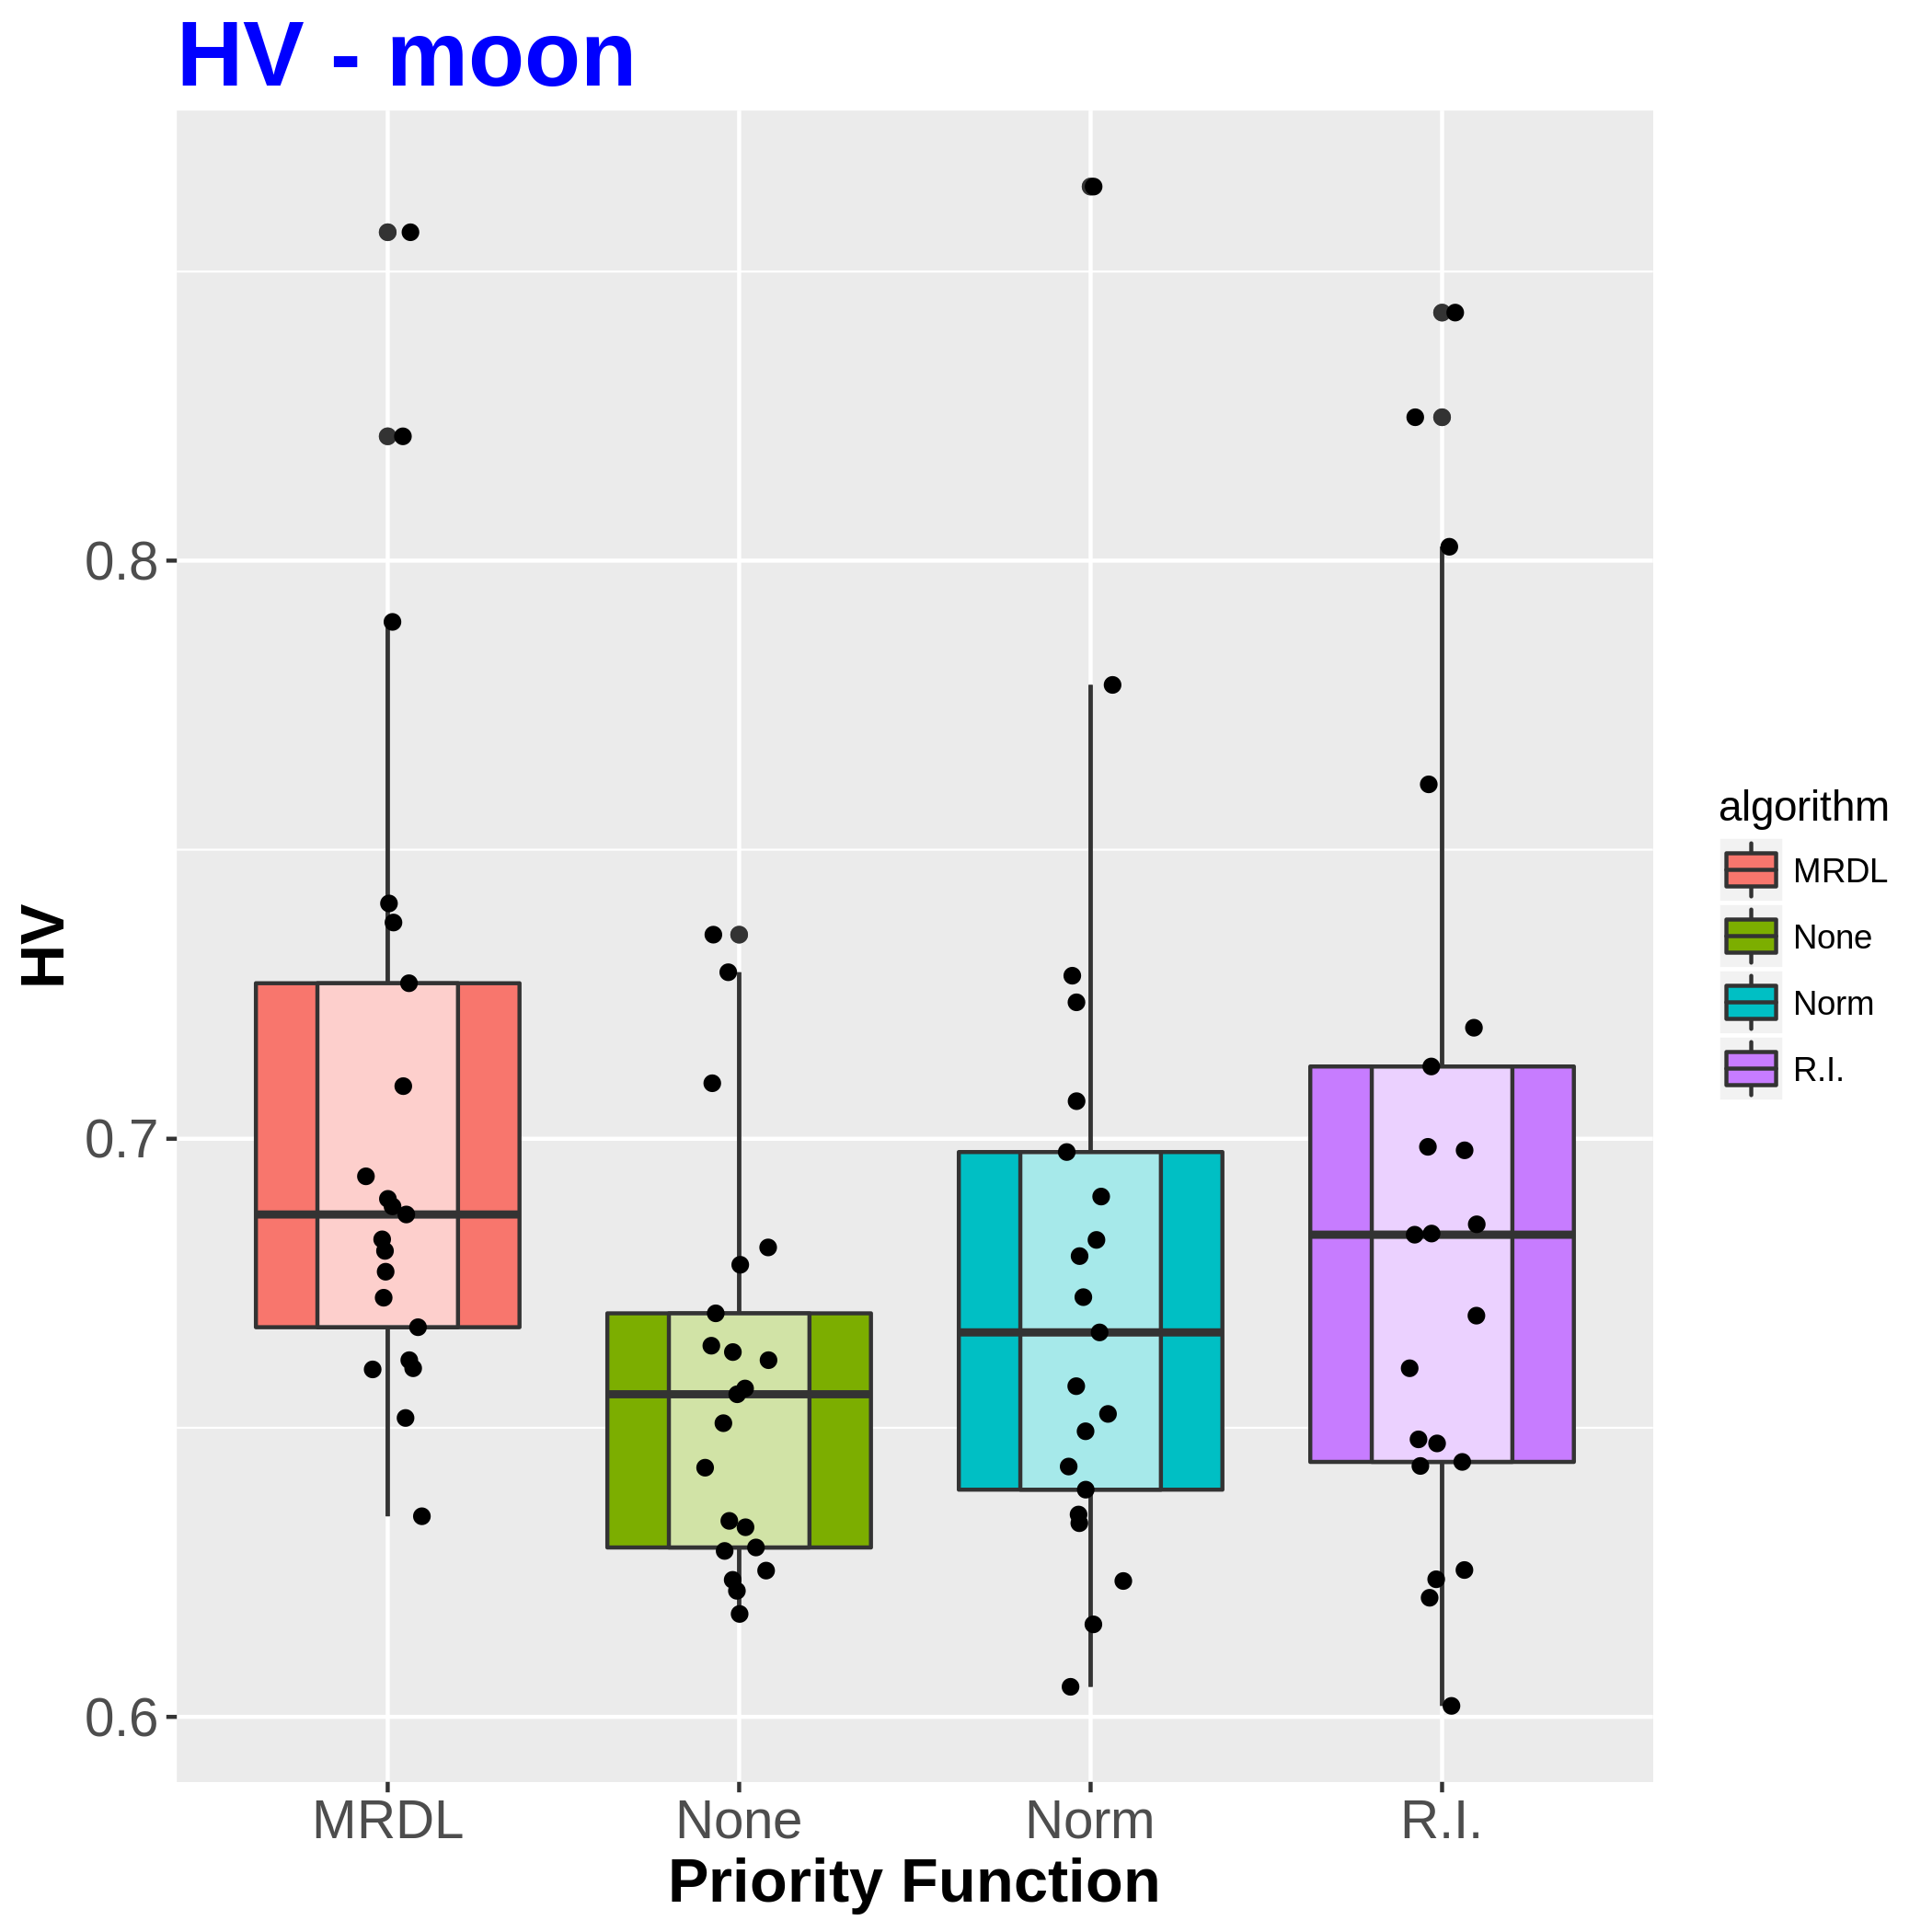
\includegraphics[width=1\textwidth, height=1\textwidth]{images/moon_HV}
		\caption{HV values of the last iteraction on the Lunar Landing Problem}
	\end{subfigure}
	\begin{subfigure}[b]{0.33\textwidth}
		\centering
	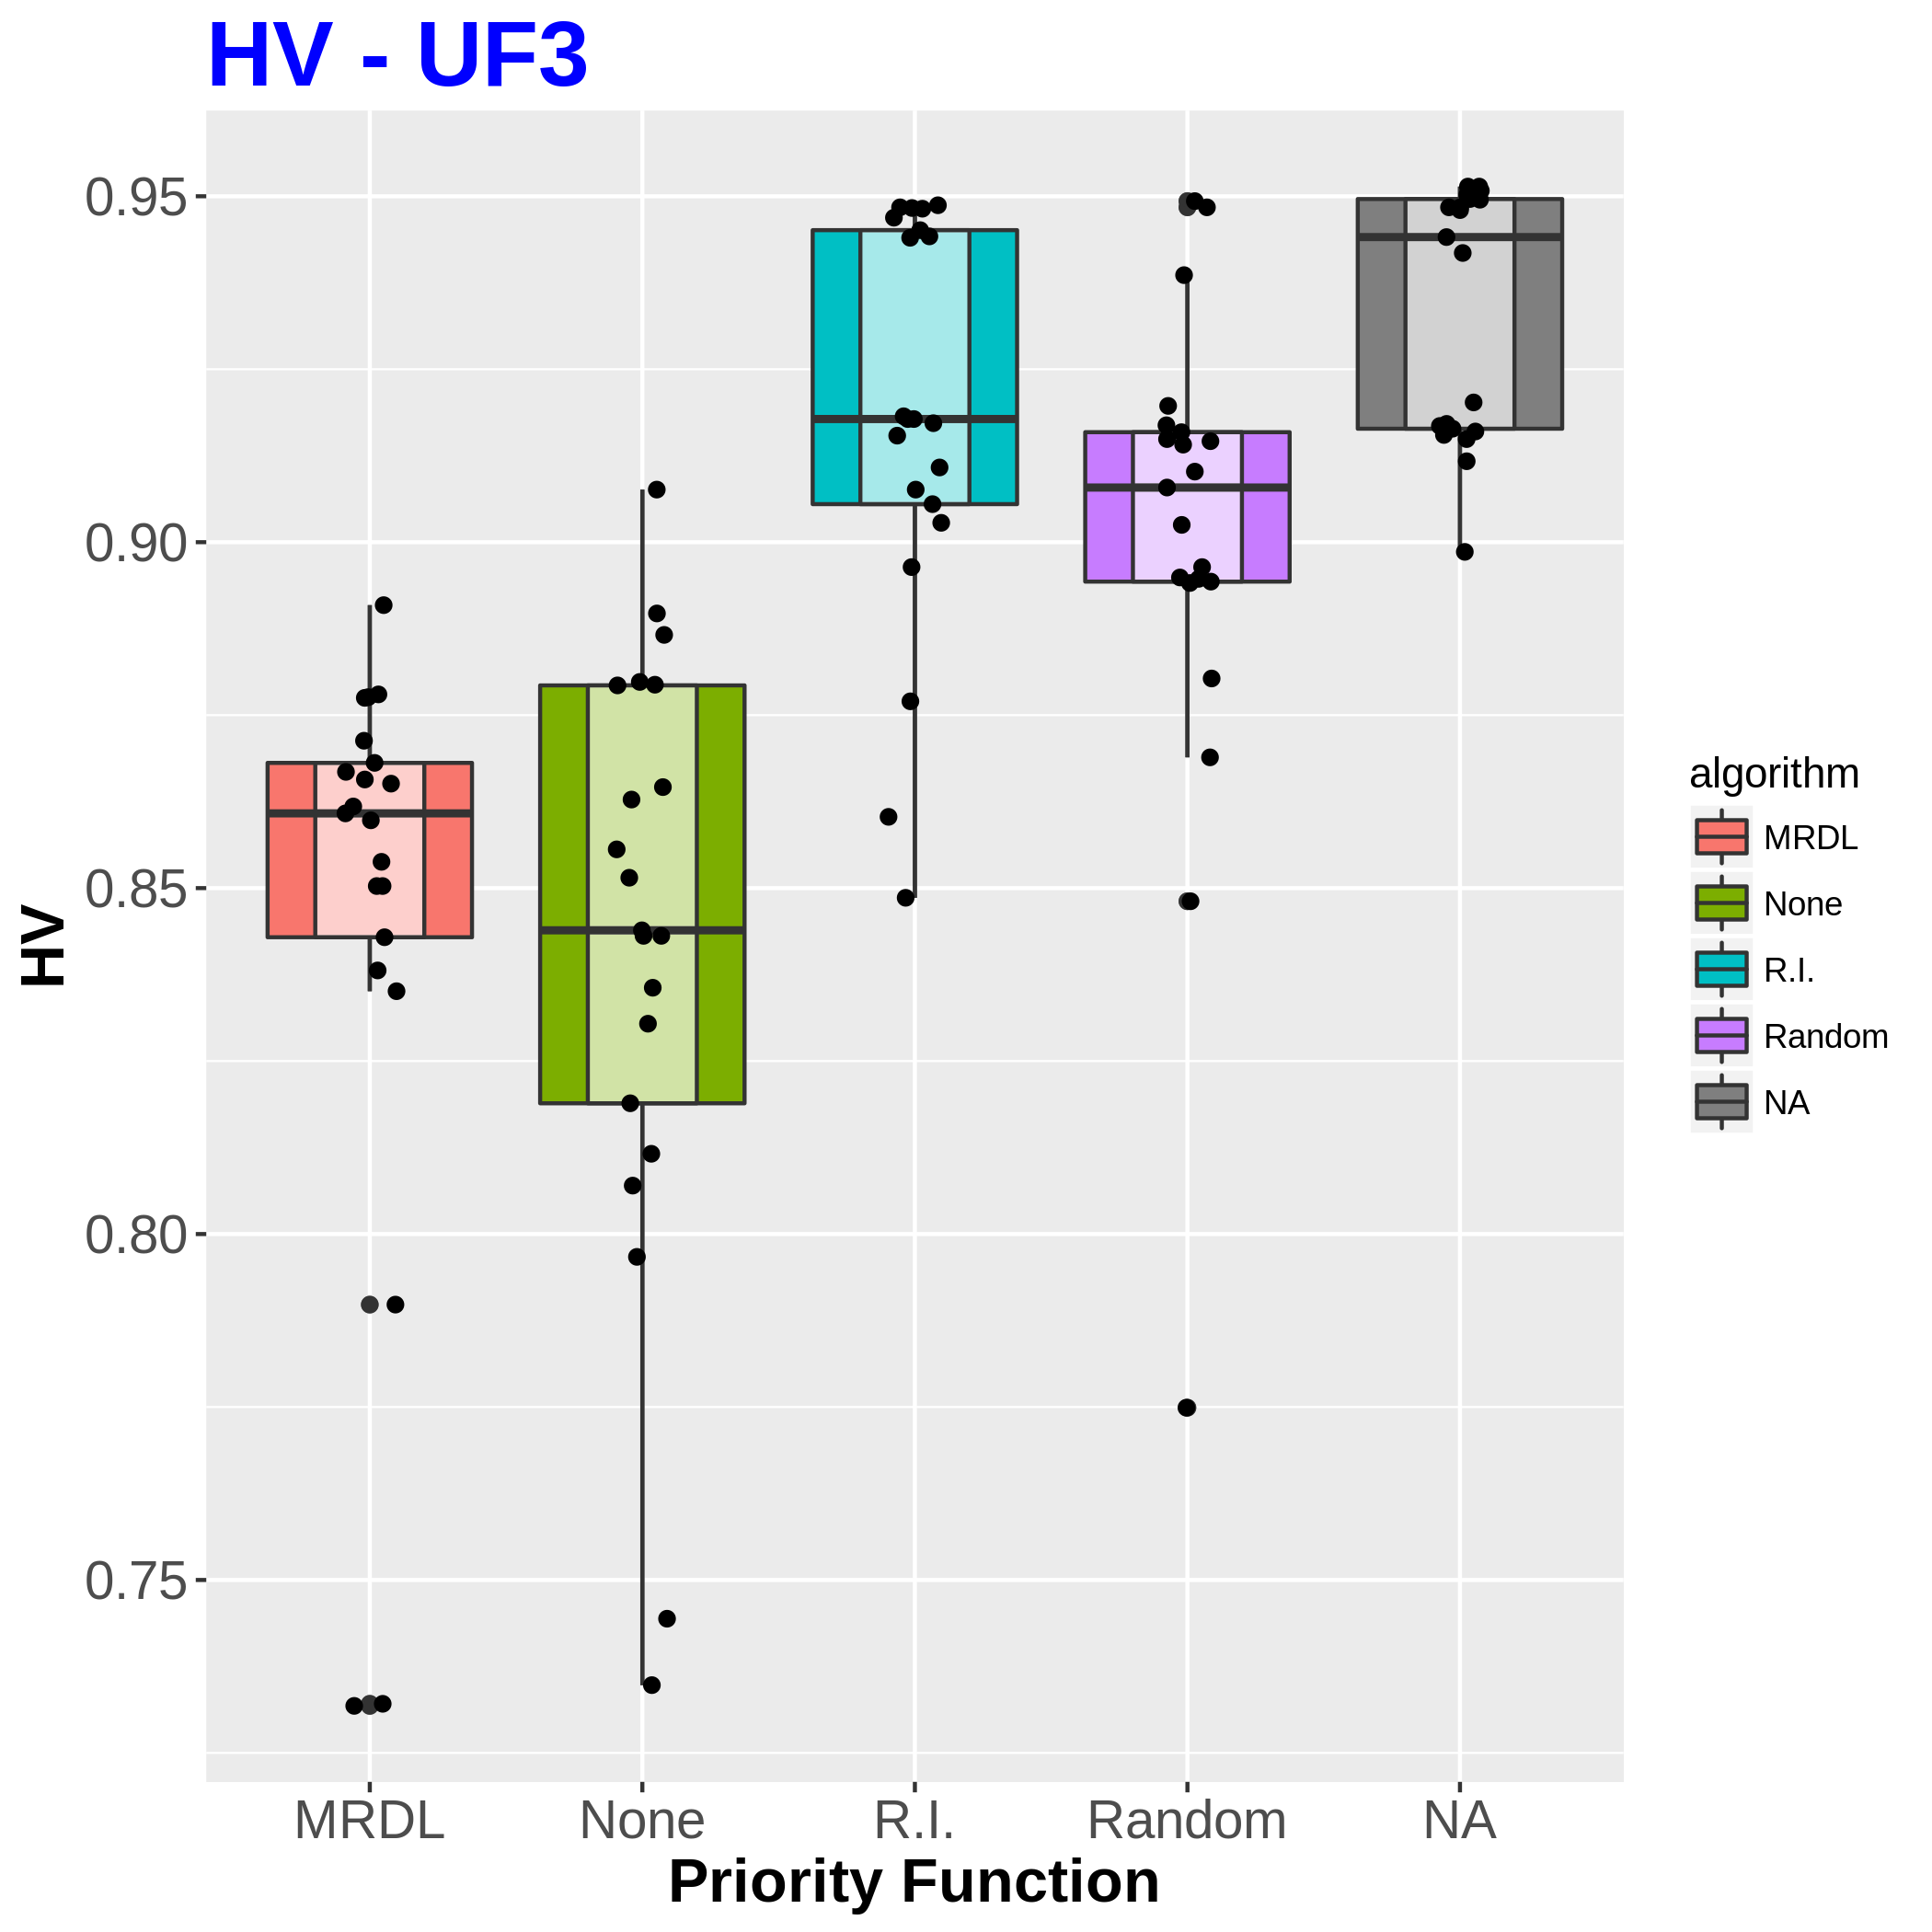
\includegraphics[width=1\textwidth, height=1\textwidth]{images/UF3_HV}
	\caption{HV values of the last iteraction on the UF-3 function Problem}
	\end{subfigure}
	\begin{subfigure}[b]{0.33\textwidth}
		\centering
	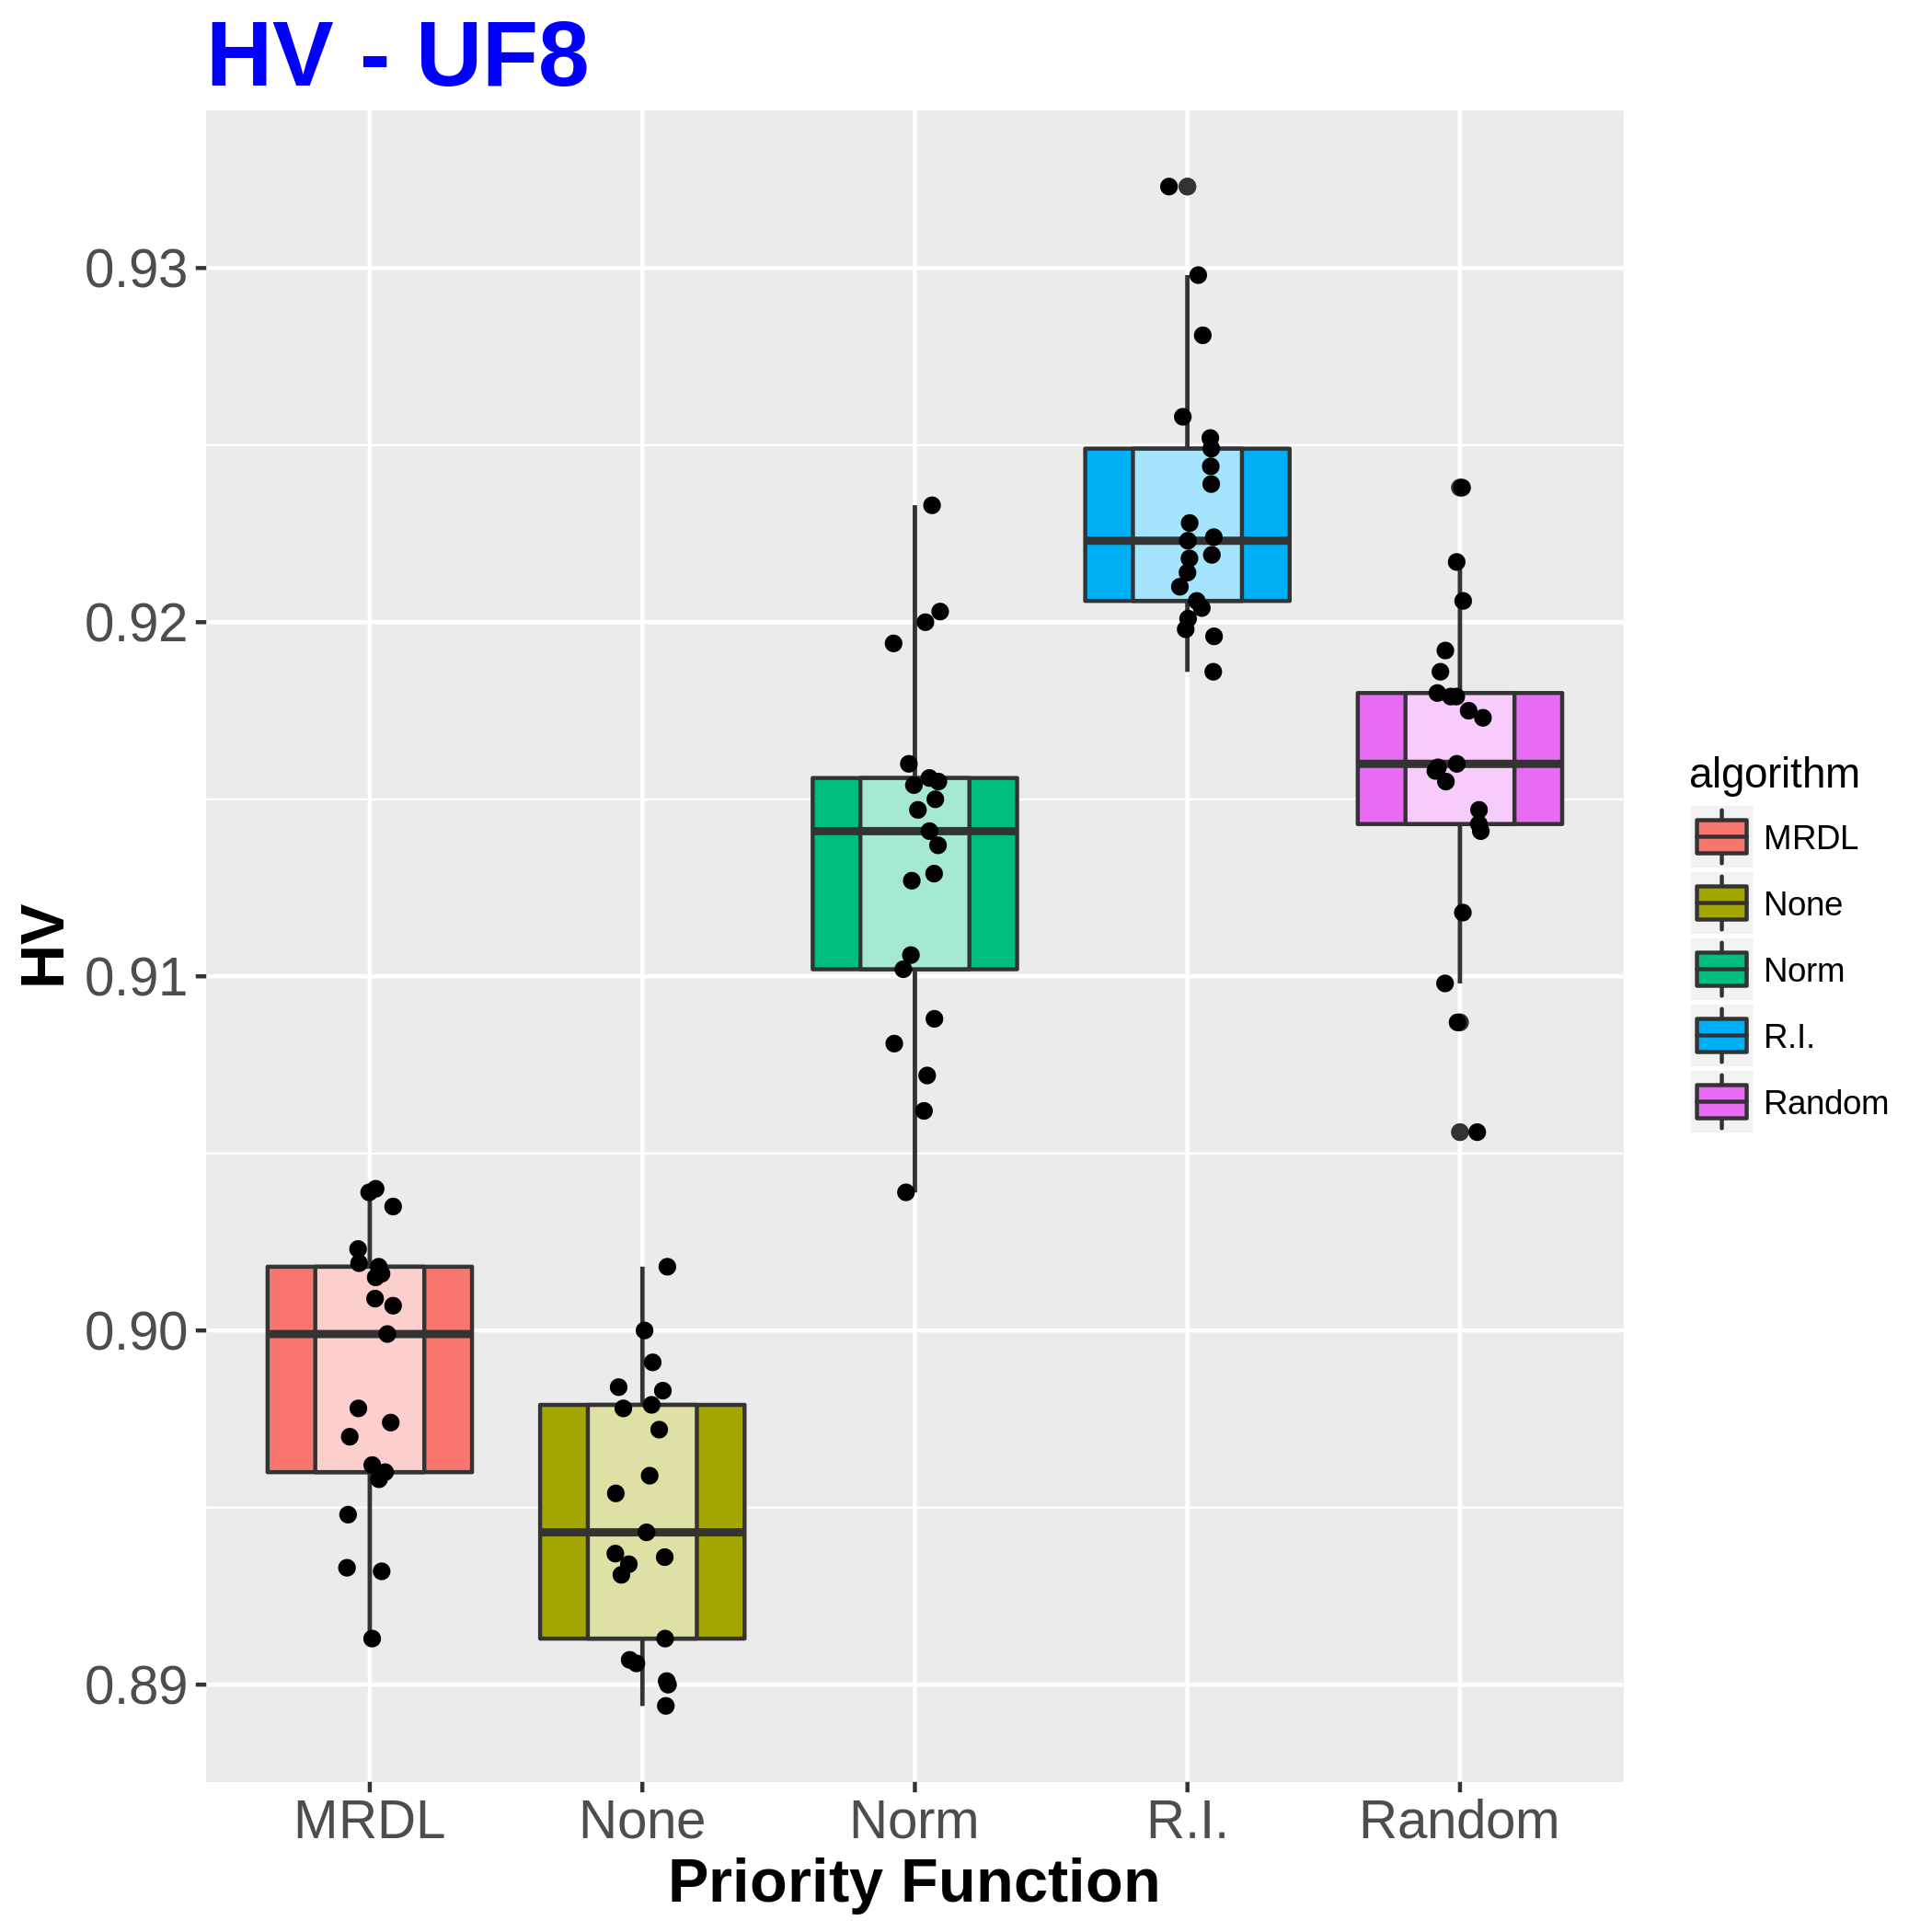
\includegraphics[width=1\textwidth, height=1\textwidth]{images/UF8_HV}
	\caption{HV values of the last iteraction on the UF-8 function Problem}
	\end{subfigure}
	\caption{SBX crossover - ($\lambda, \lambda$) scheme.}
		\label{HVS}
\end{figure*}

\begin{figure*}[!t]
%	\Large{Average performance on different tournament size - Gallagher's Gaussian 21-hi Peaks Function}
	\begin{subfigure}[b]{0.33\textwidth}
		\centering
		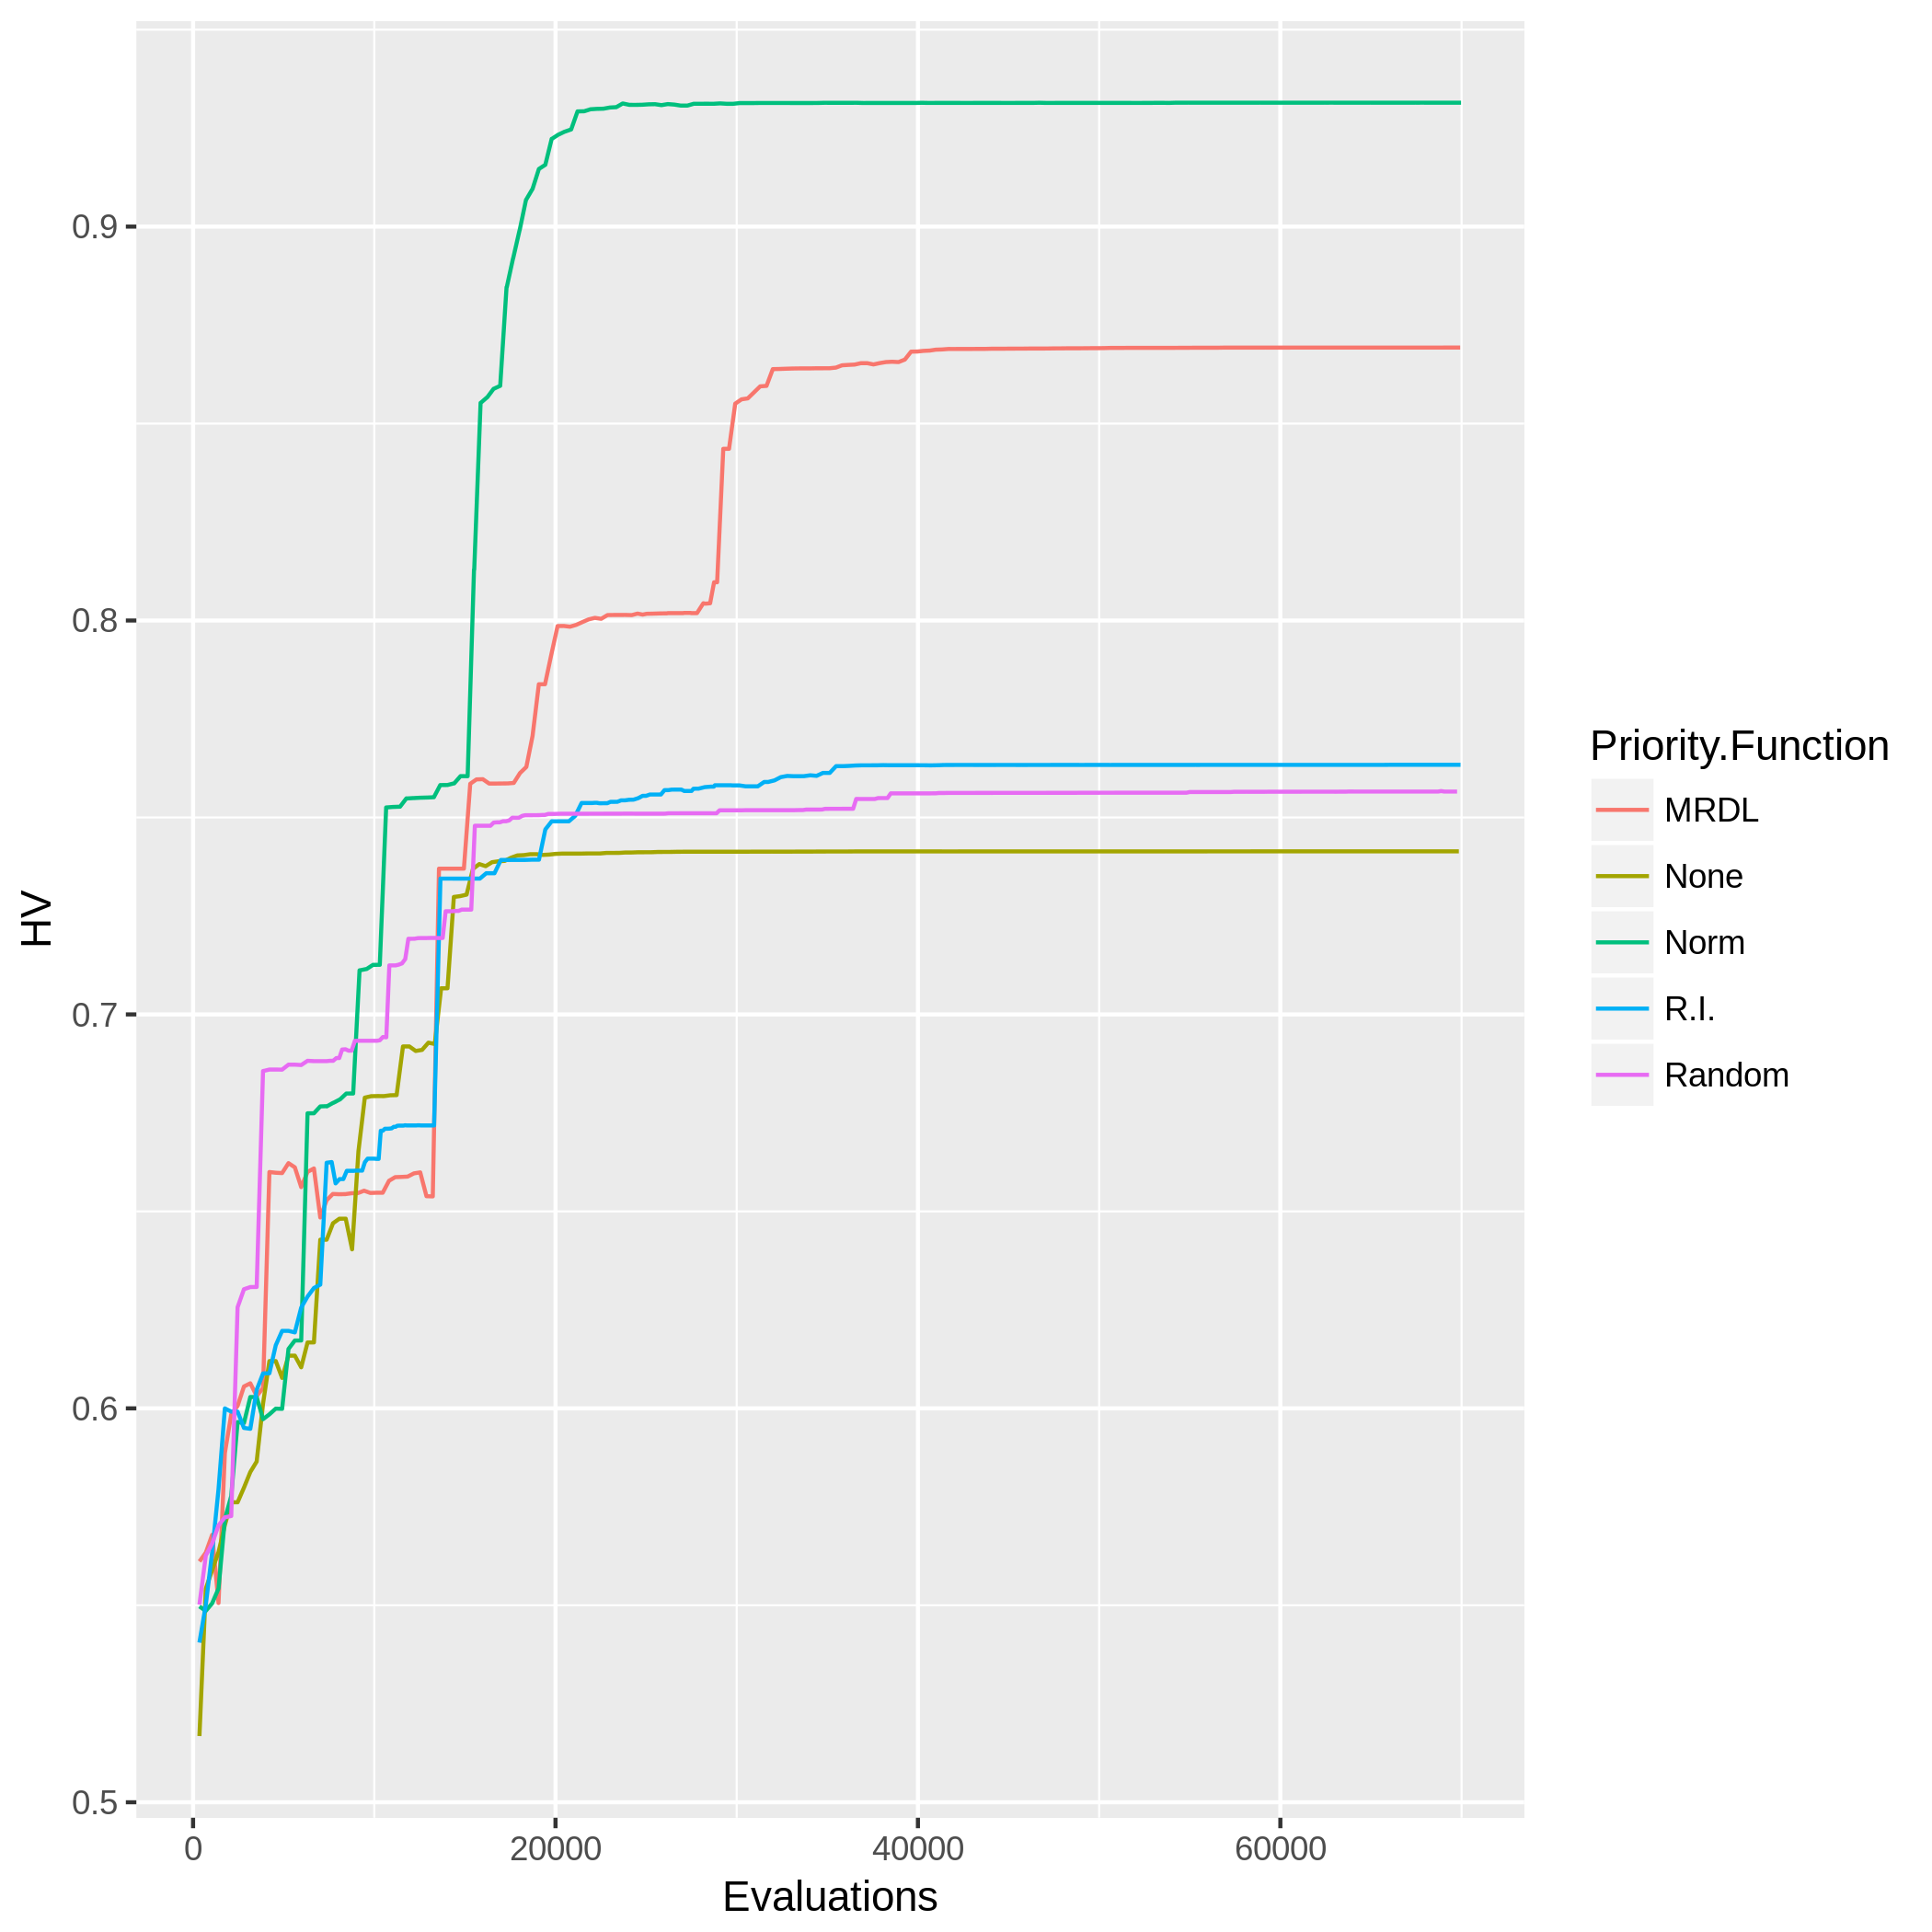
\includegraphics[width=1\textwidth, height=1\textwidth]{images/moonhv_all}
		\caption{Evolution of the HV on the Lunar Landing}
	\end{subfigure}
	\begin{subfigure}[b]{0.33\textwidth}
		\centering
		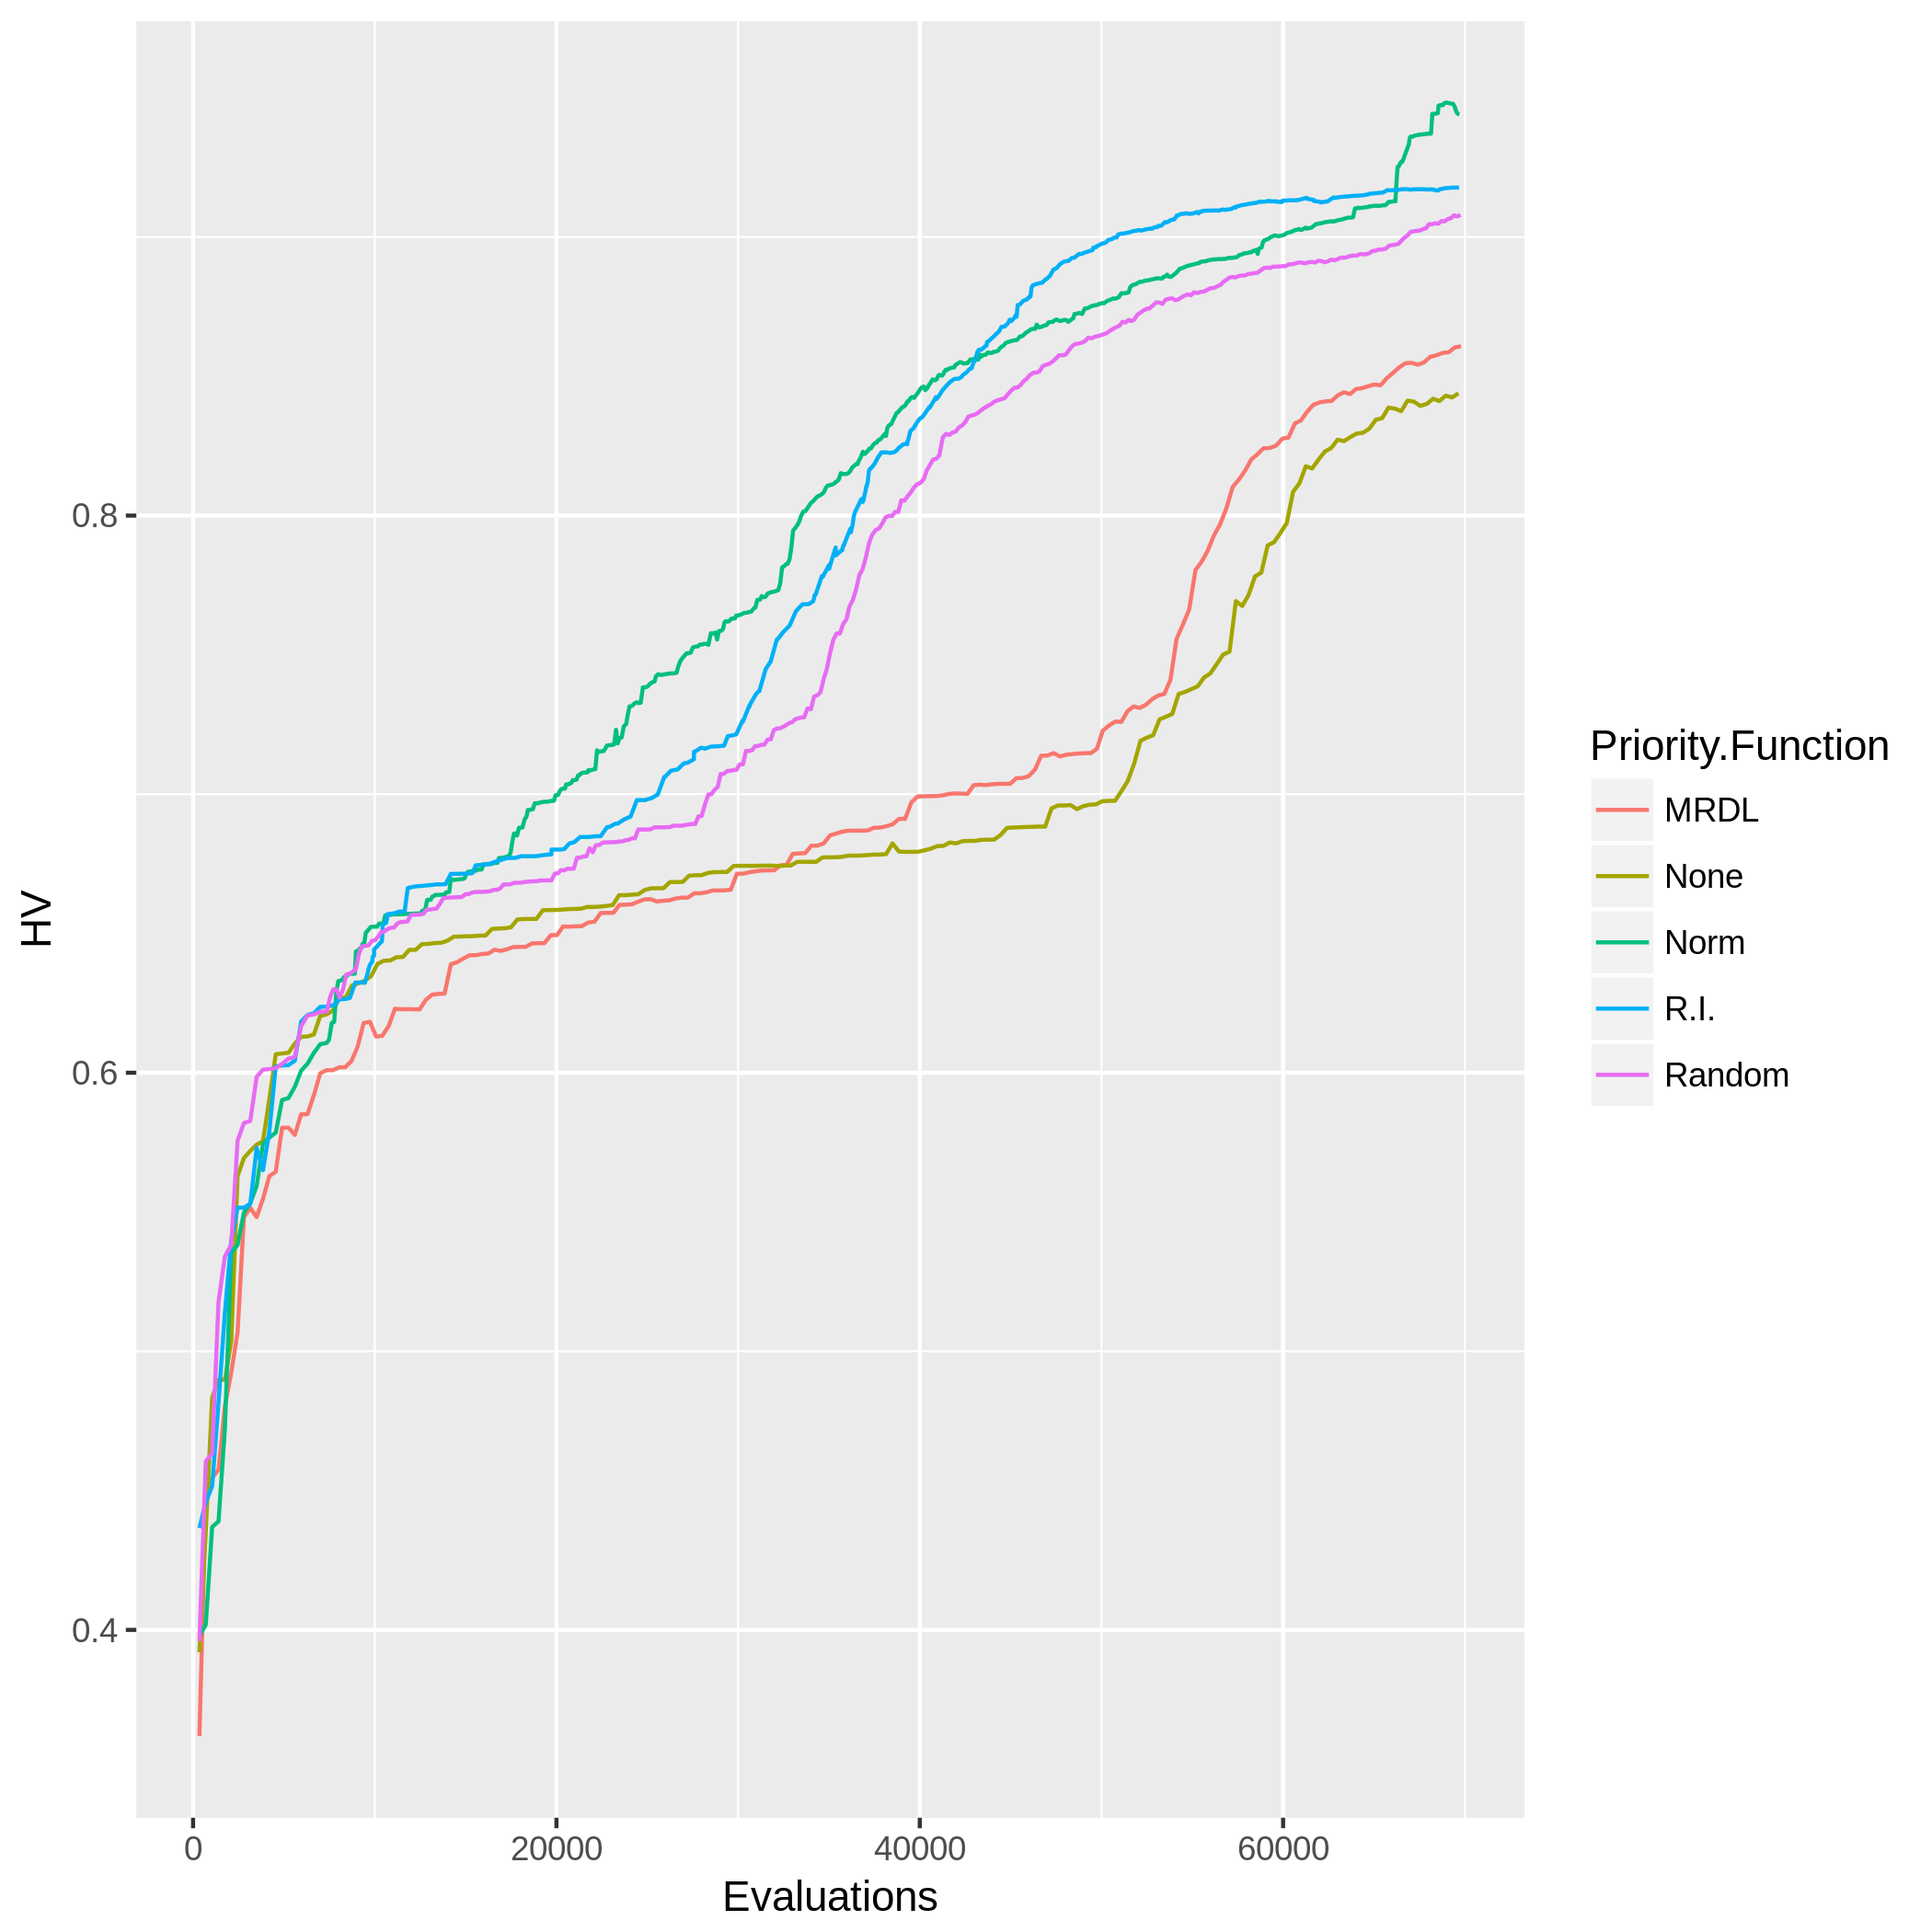
\includegraphics[width=1\textwidth, height=1\textwidth]{images/UF3hv_all}
		\caption{Evolution of the HV on the UF3}
	\end{subfigure}
	\begin{subfigure}[b]{0.33\textwidth}
		\centering
		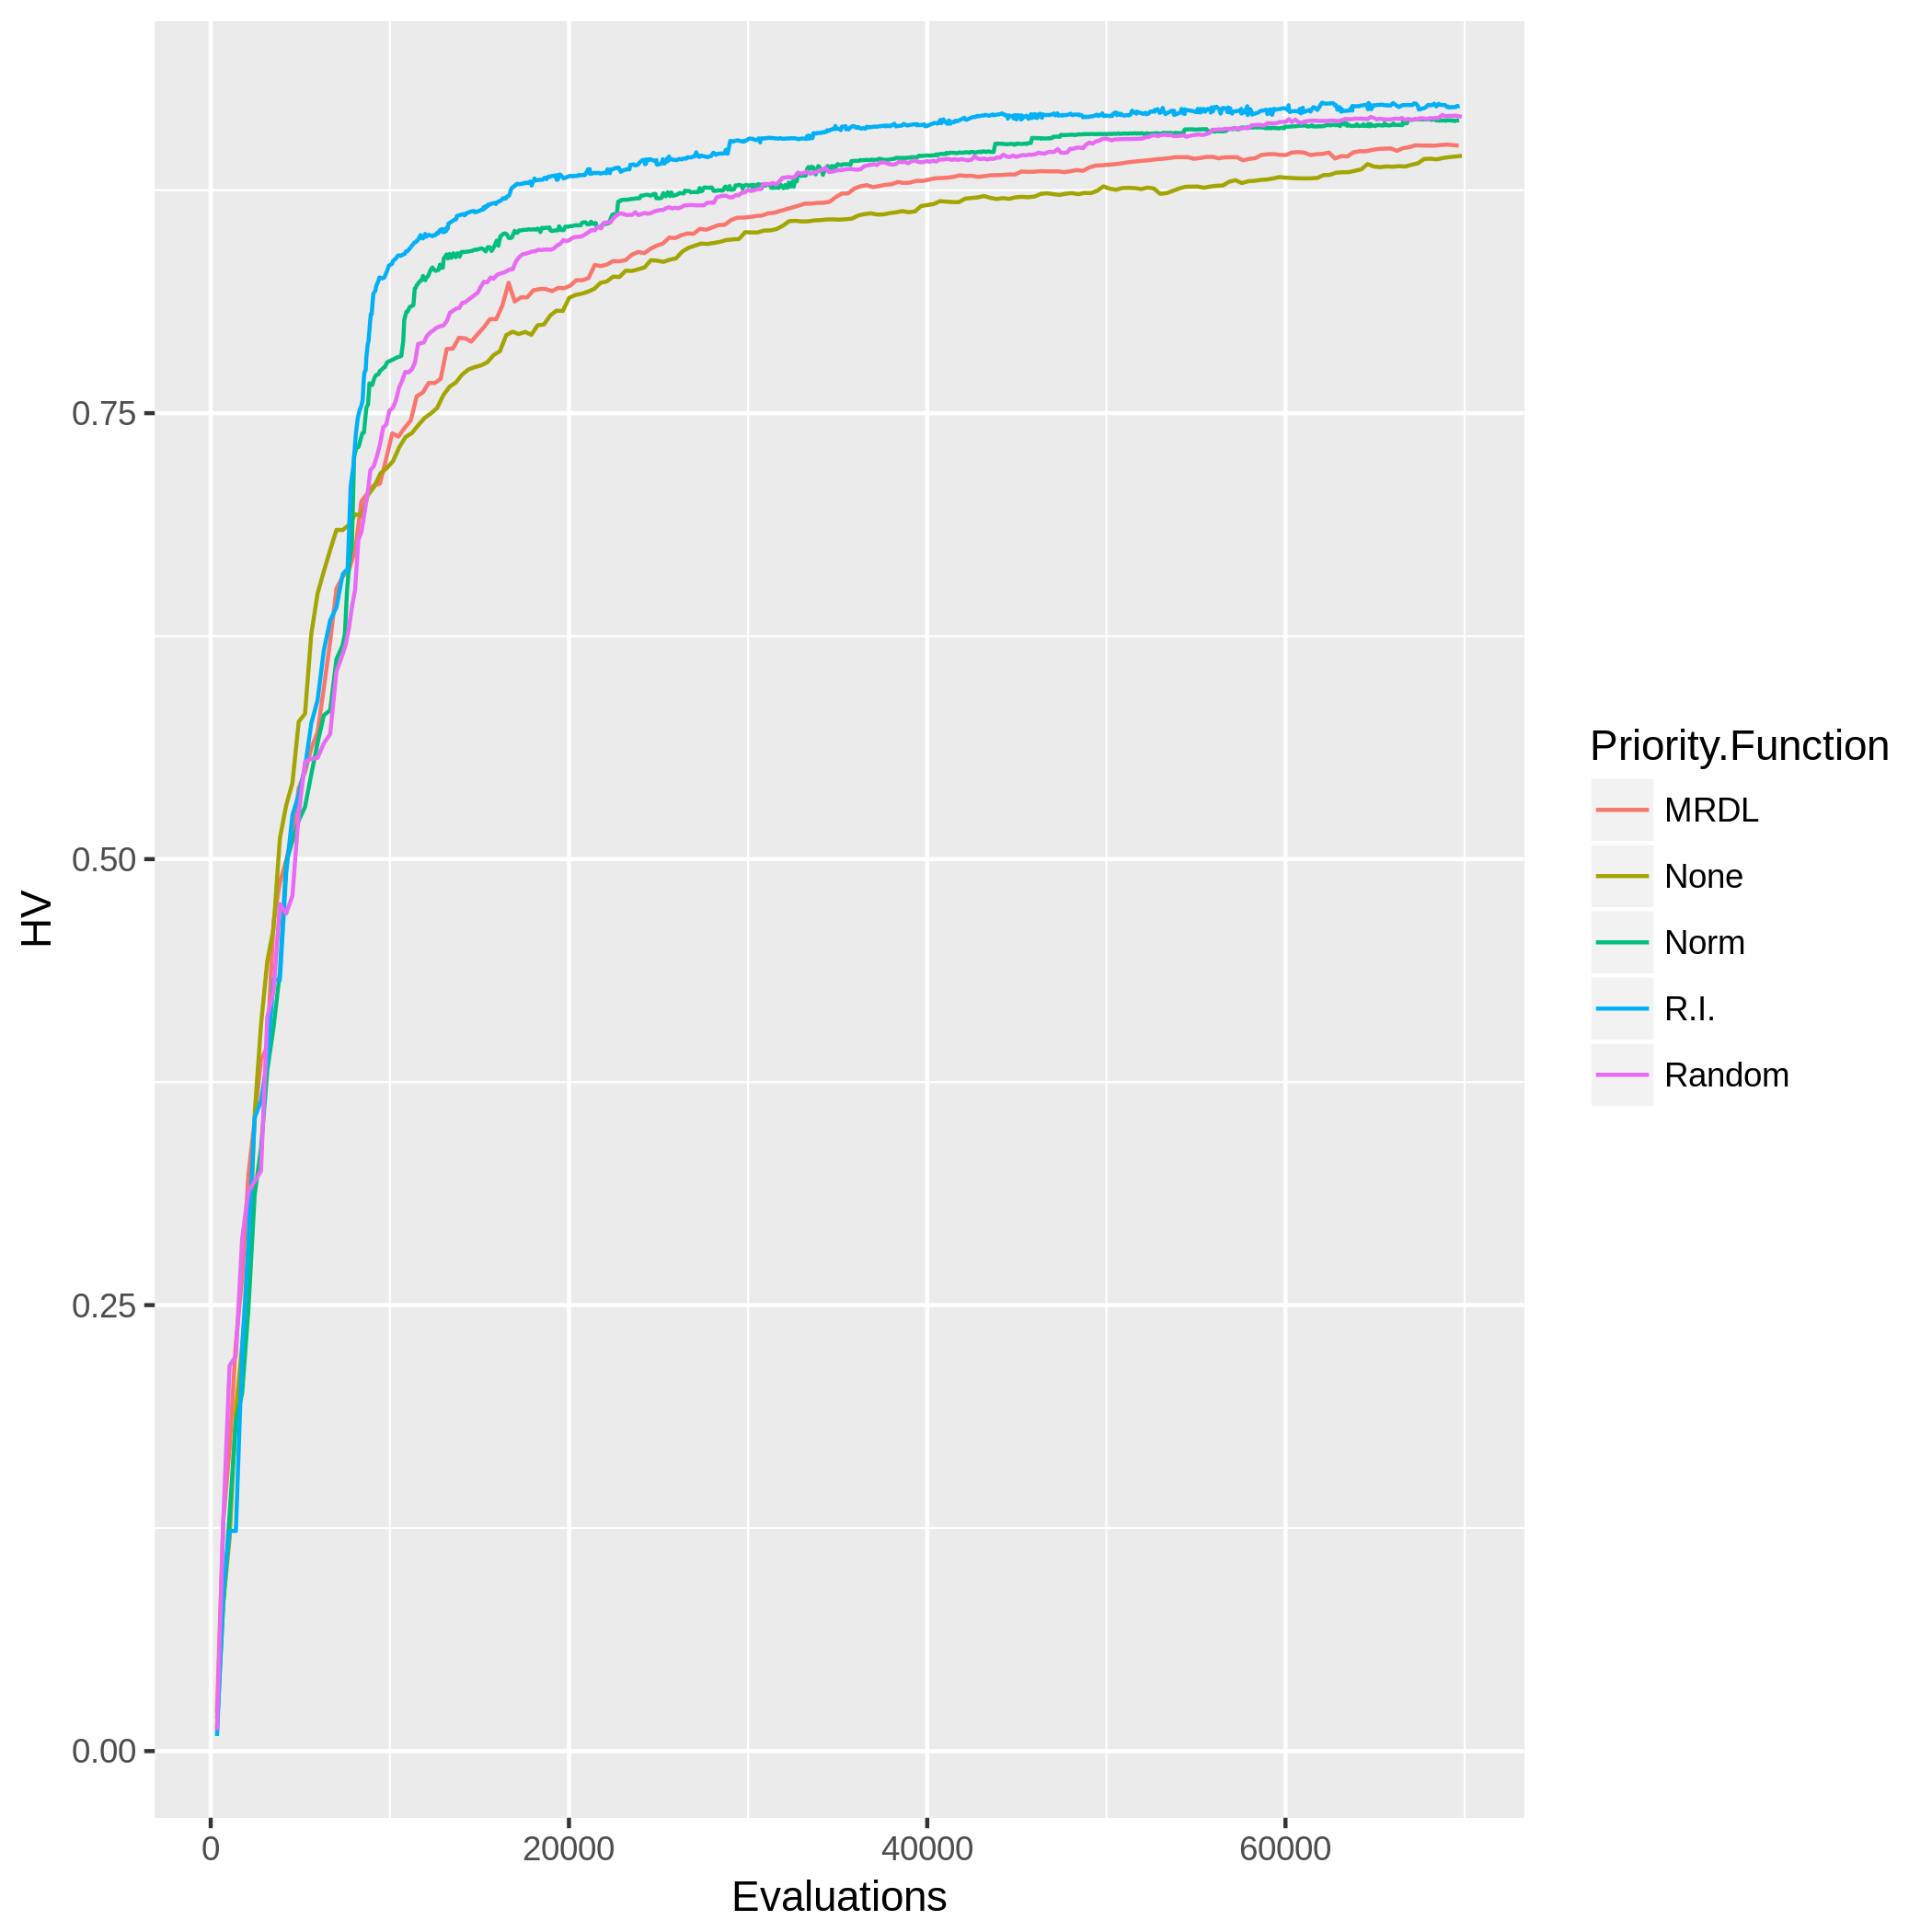
\includegraphics[width=1\textwidth, height=1\textwidth]{images/UF8hv_all}
		\caption{Evolution of the HV on the UF8}
	\end{subfigure}
	\caption{SBX crossover - ($\lambda, \lambda$) scheme.}
\label{evolution_hv}
\end{figure*}

\begin{figure*}[!t]

	\begin{subfigure}[b]{0.49\textwidth}
		\centering
		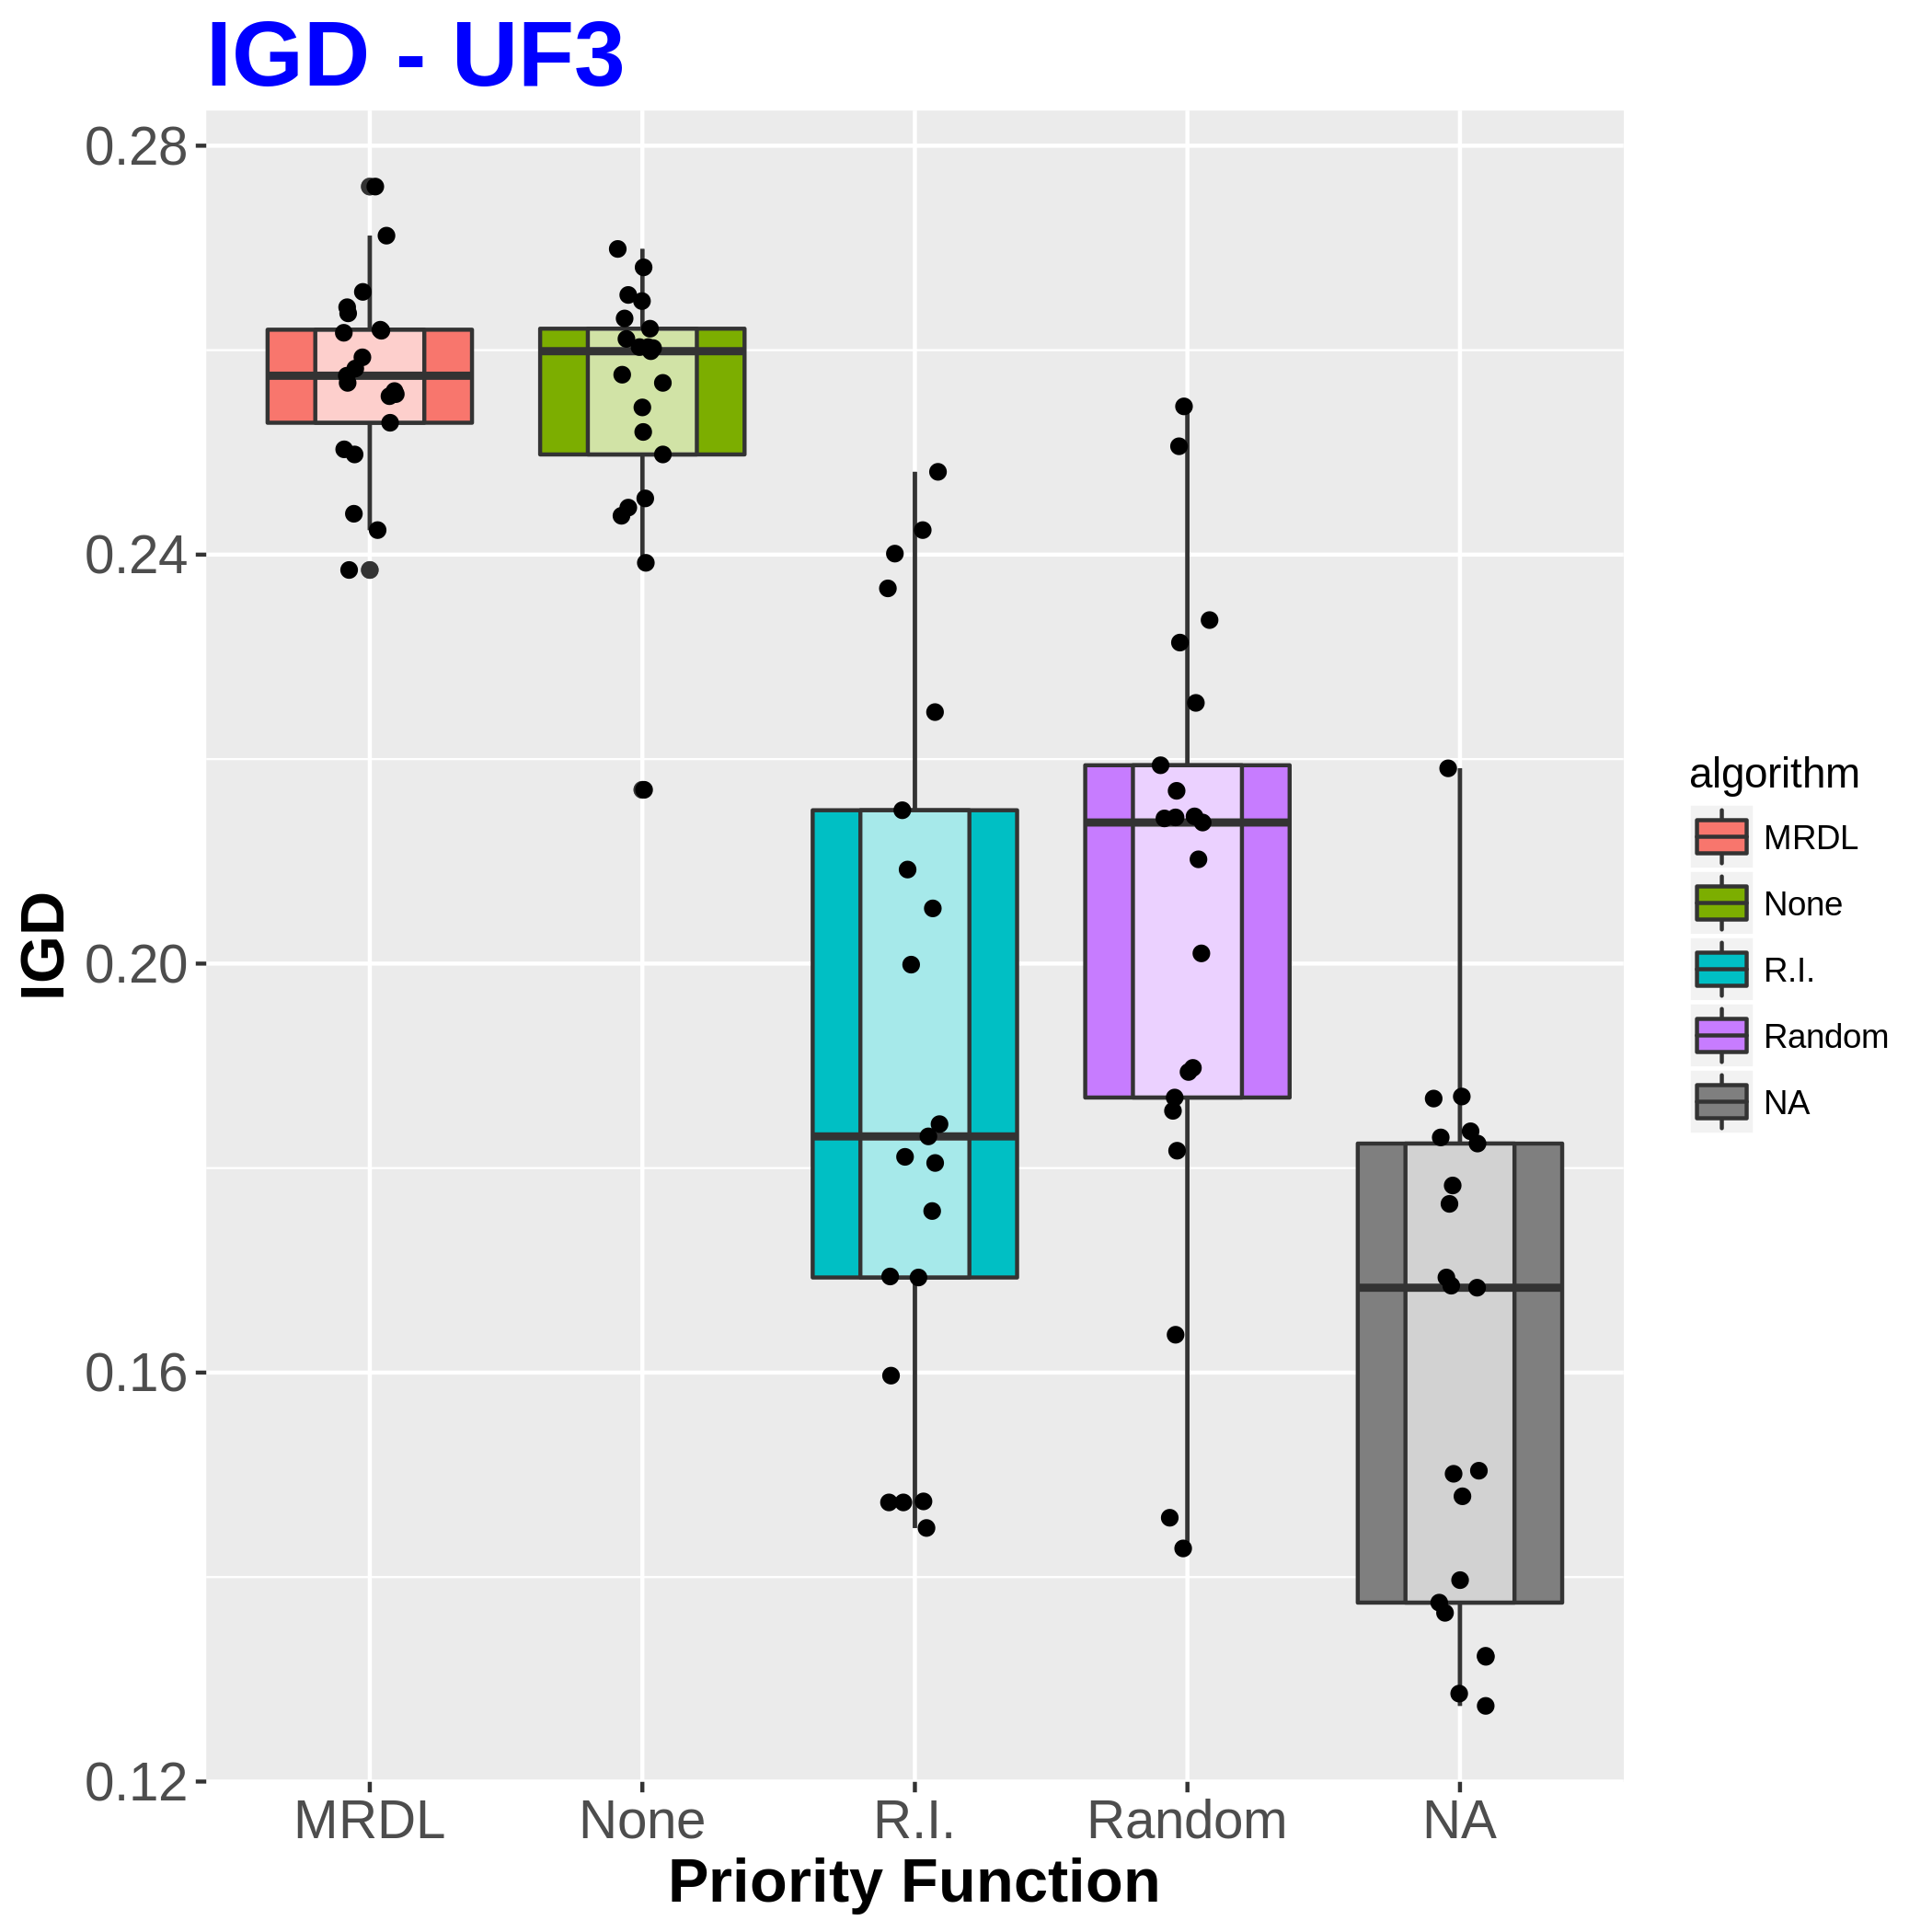
\includegraphics[width=1\textwidth, height=0.7\textwidth]{images/UF3_IGD}
		\caption{IGD values of the last iteraction on the UF-3 function}
	\end{subfigure}
	\begin{subfigure}[b]{0.49\textwidth}
		\centering
		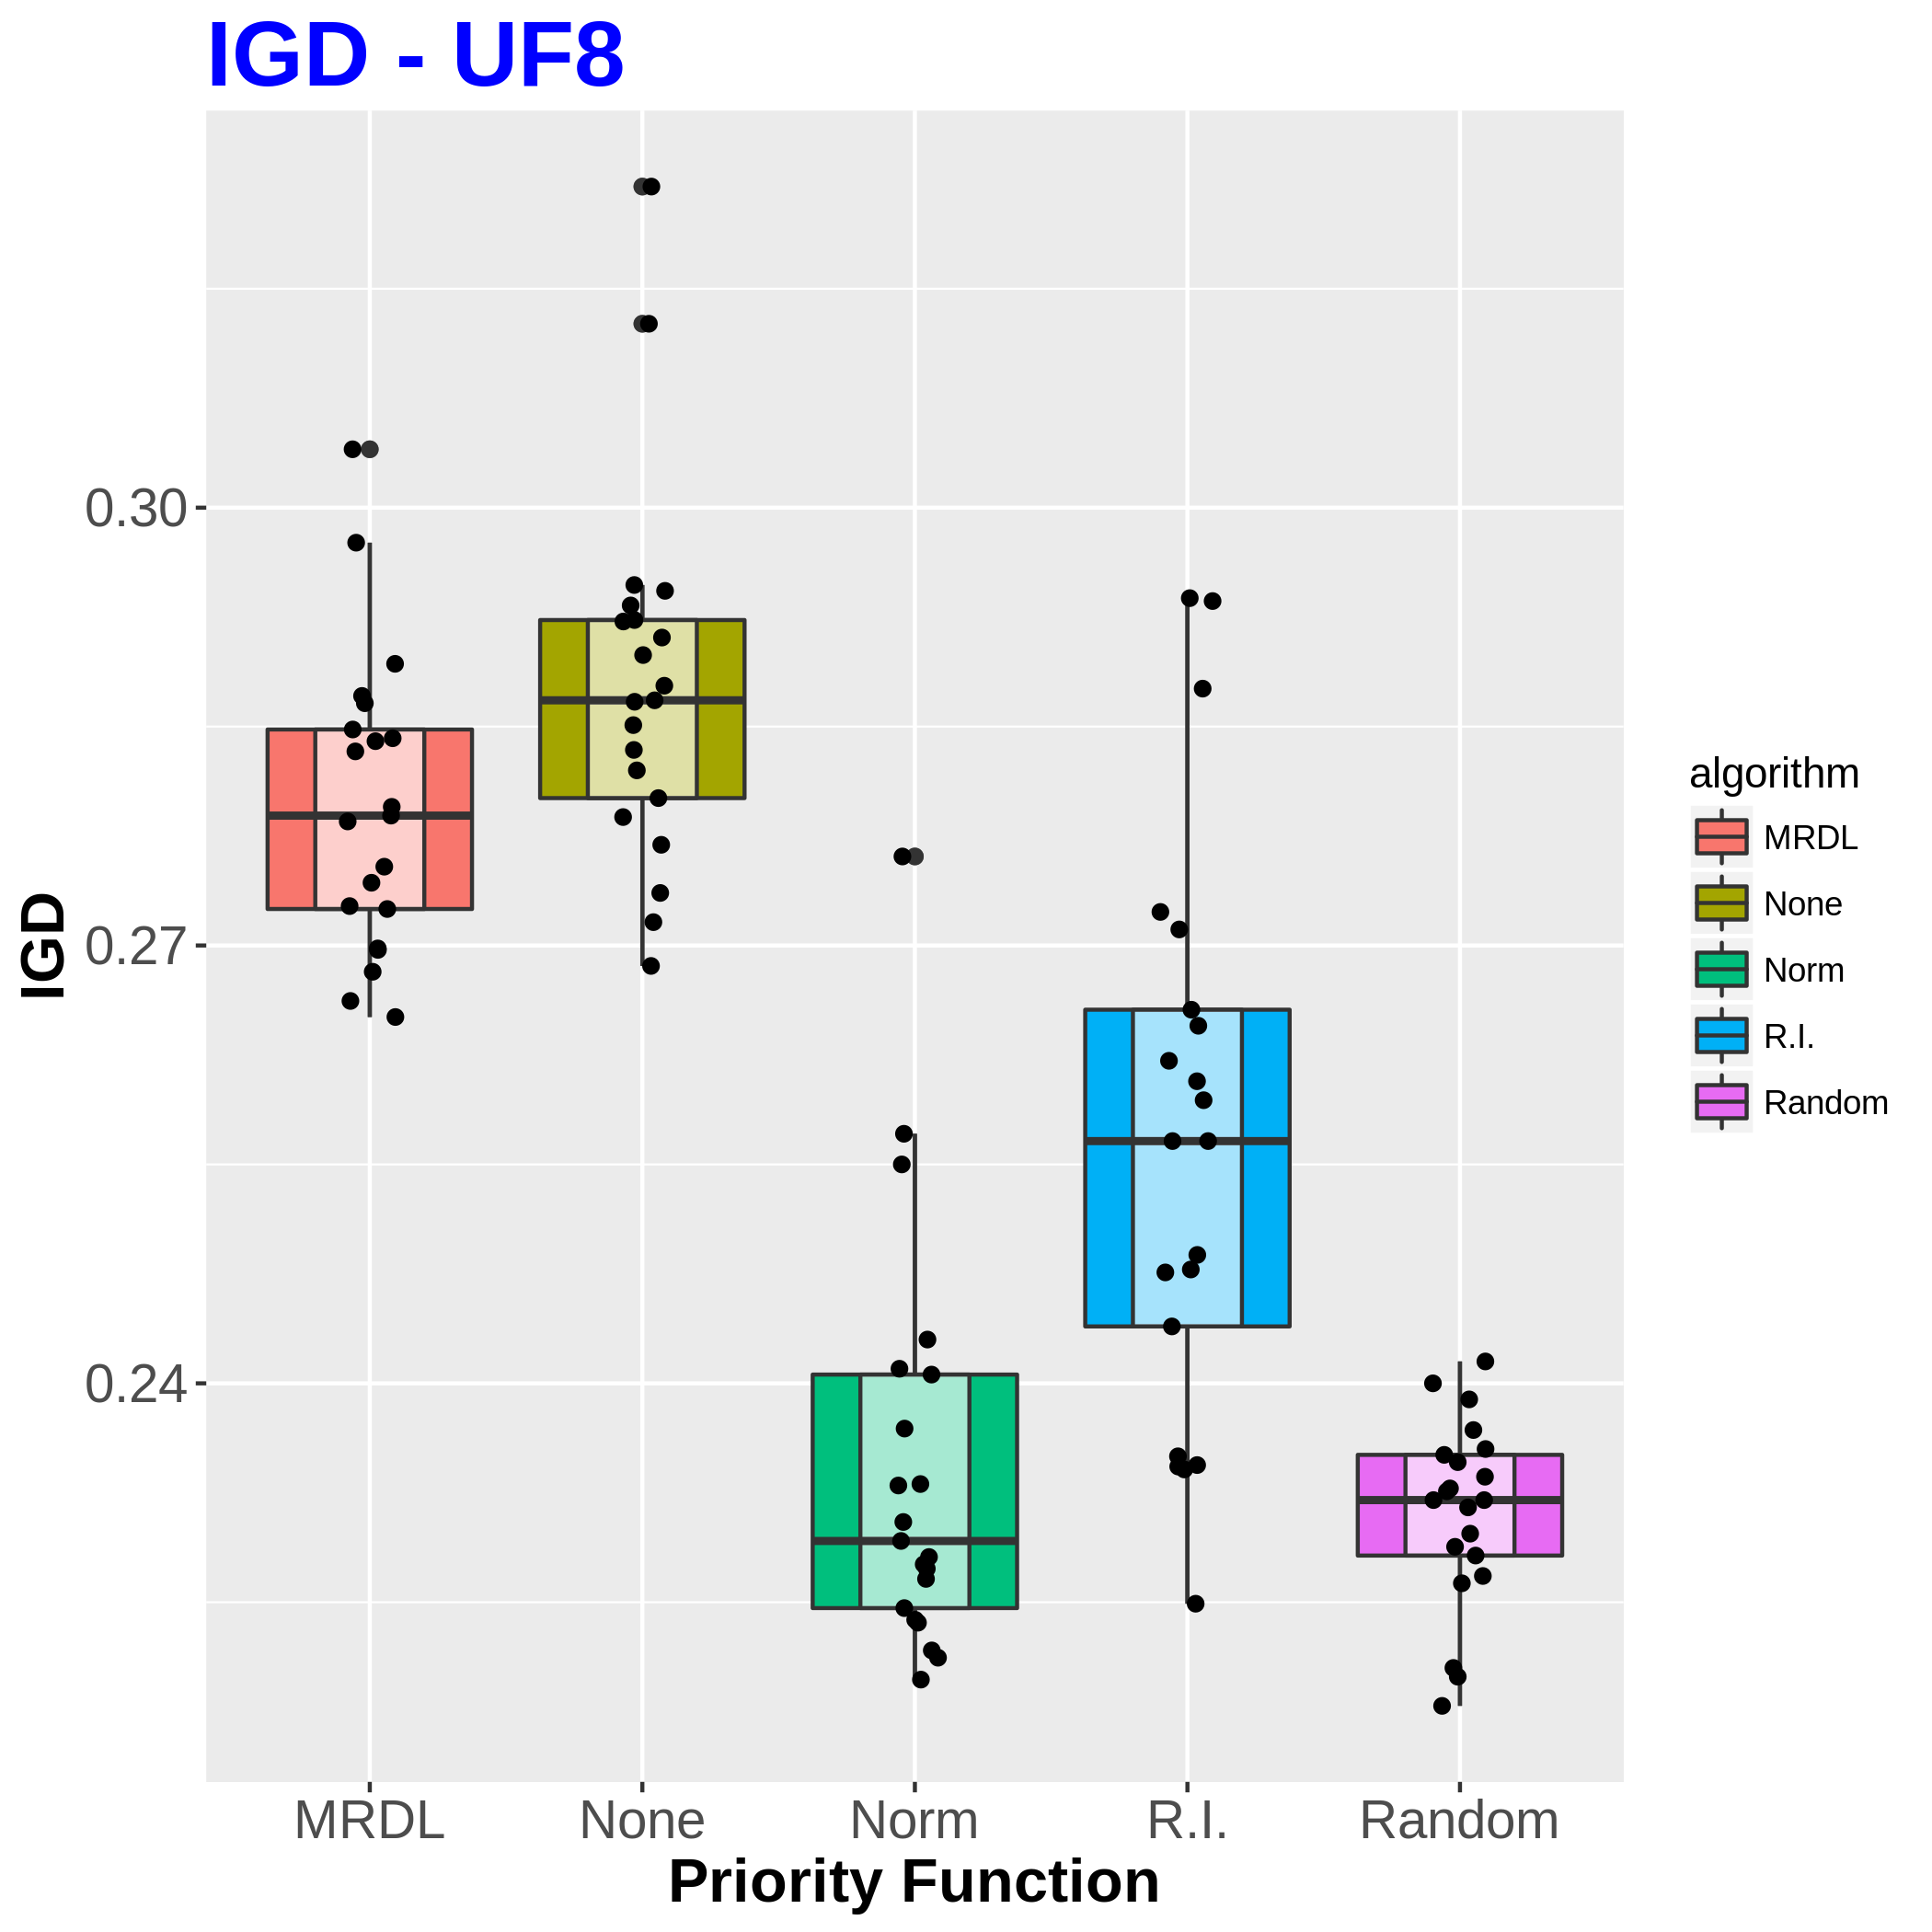
\includegraphics[width=1\textwidth, height=0.7\textwidth]{images/UF8_IGD}
		\caption{IGD values of the last iteraction on the UF-3 function}
	\end{subfigure}
	\caption{SBX crossover - ($\lambda, \lambda$) scheme.}
		\label{IGDS}
\end{figure*}



\begin{figure*}[!t]

		\begin{subfigure}[b]{0.49\textwidth}
			\centering
		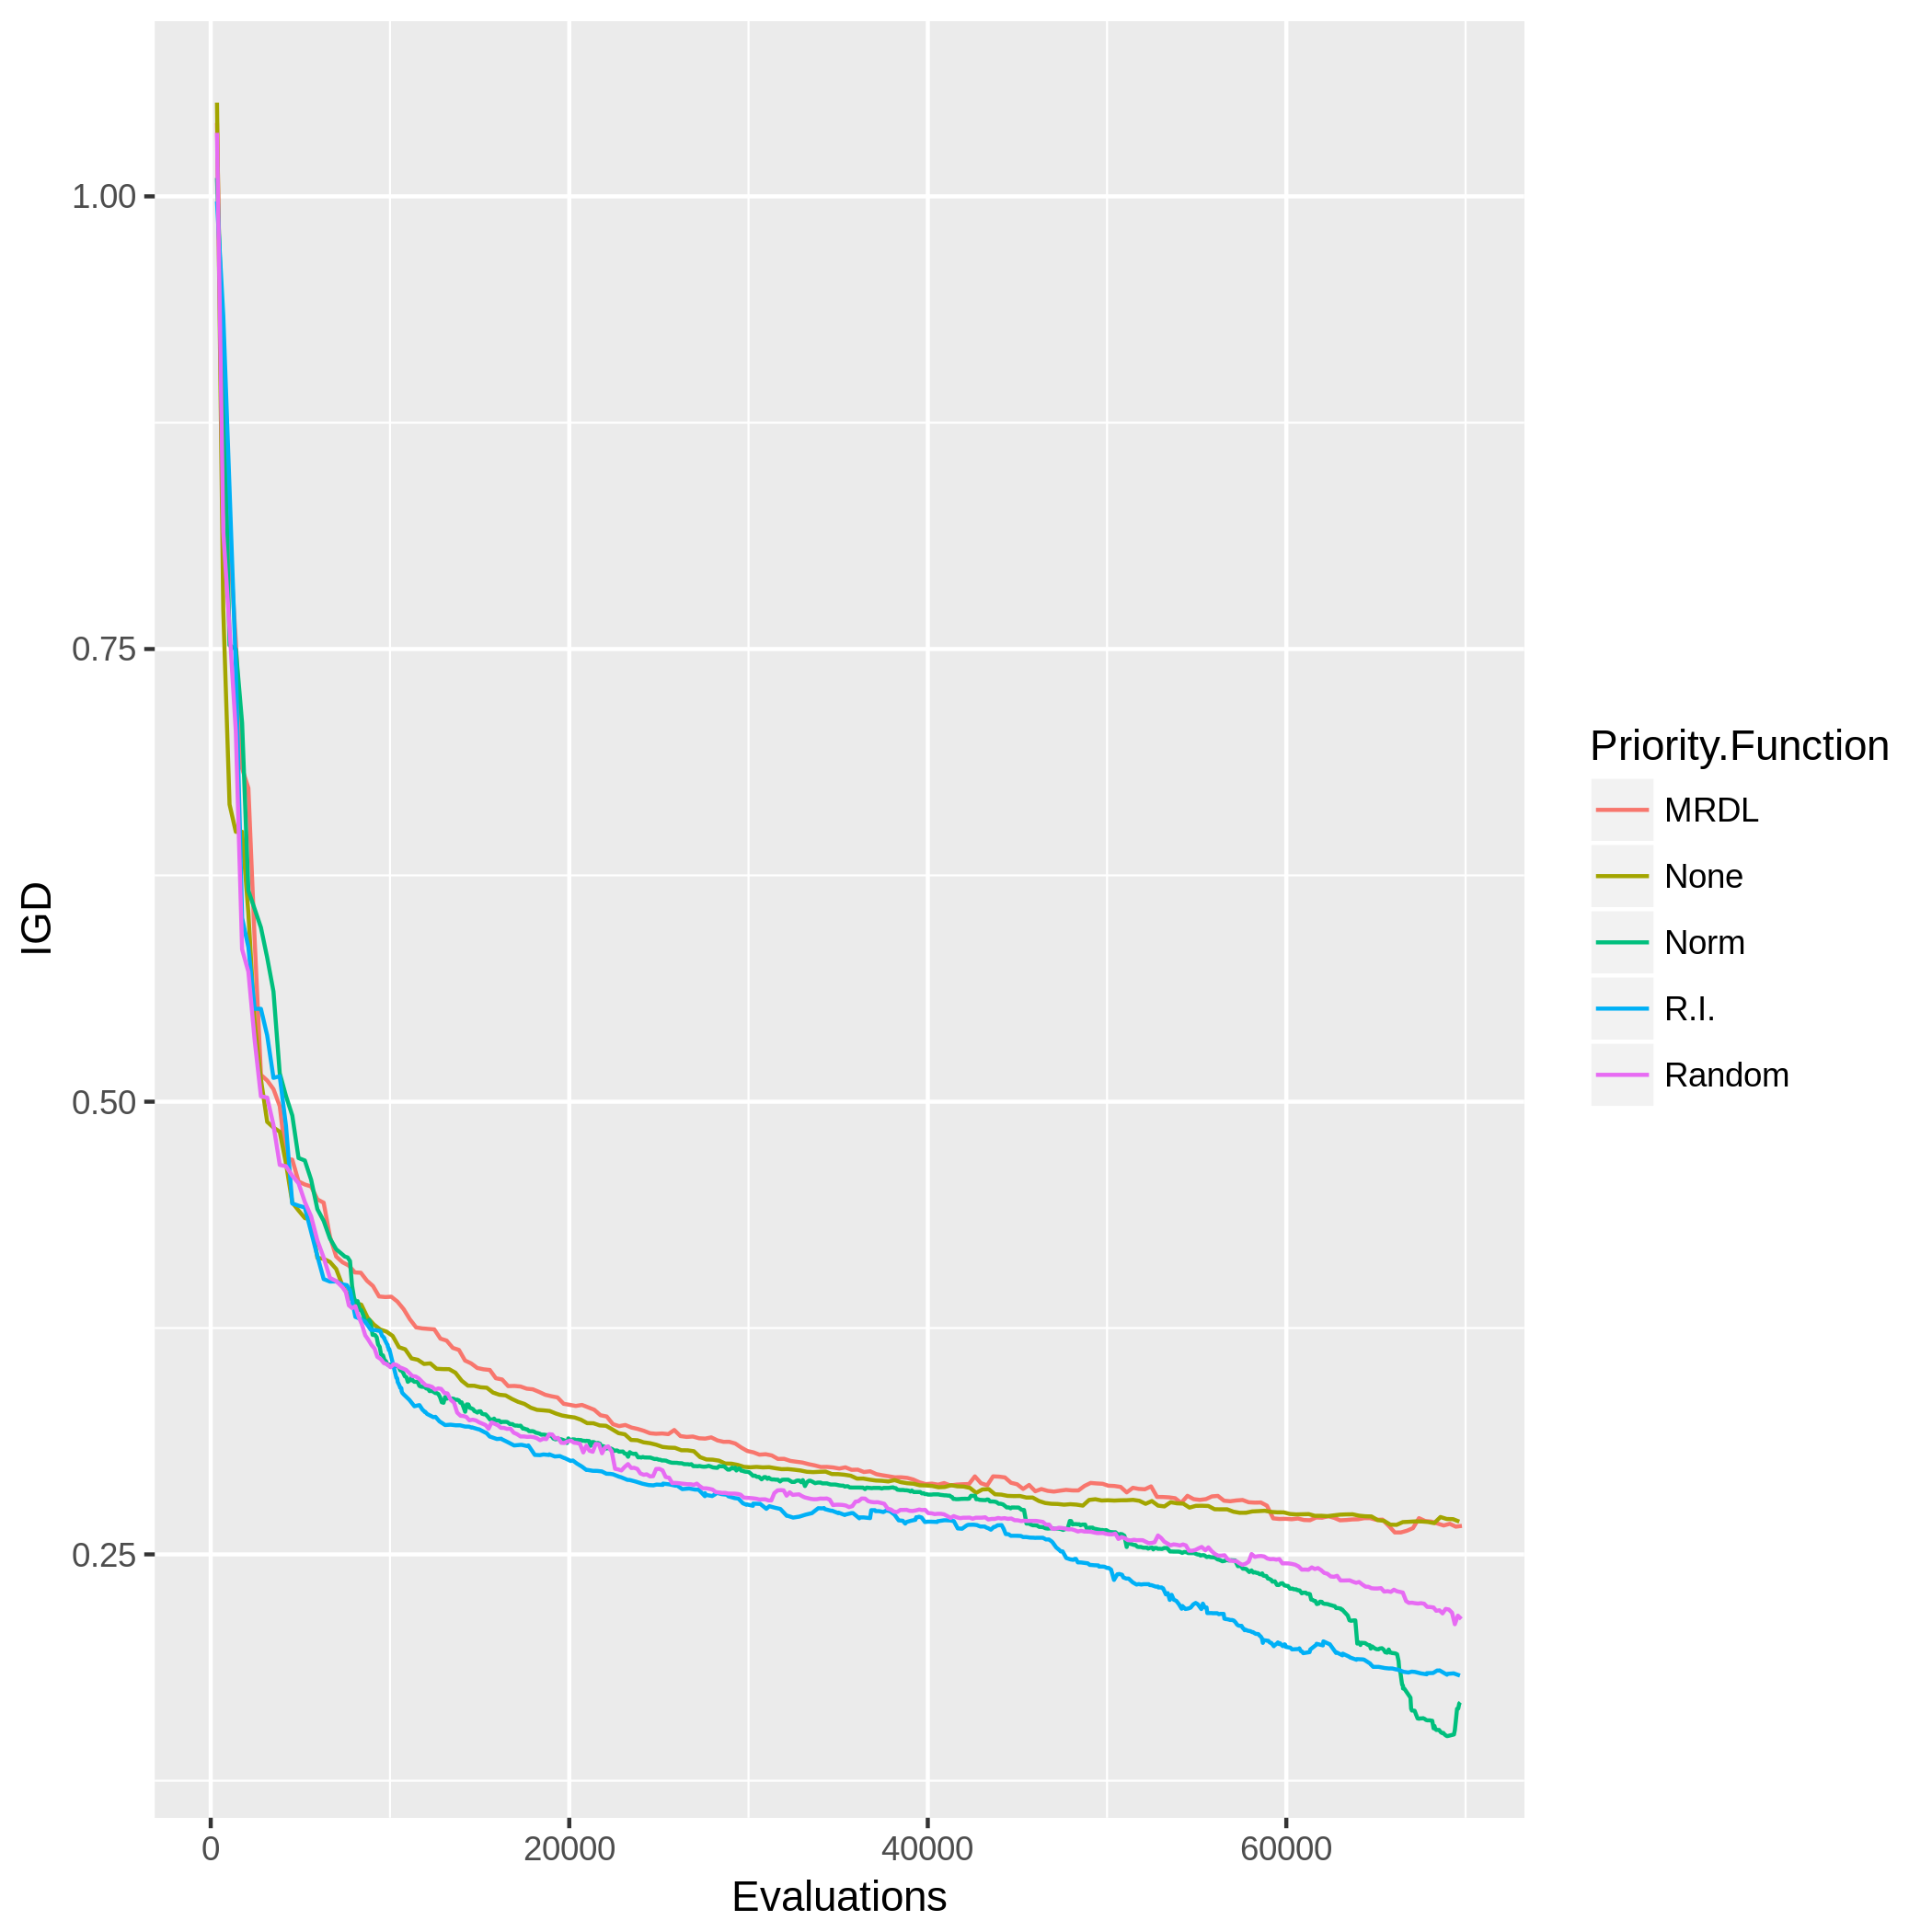
\includegraphics[width=1\textwidth, height=0.7\textwidth]{images/UF3igd_all}
			\caption{Evolution of the IGD on the UF3}
		\end{subfigure}
		\begin{subfigure}[b]{0.49\textwidth}
			\centering
		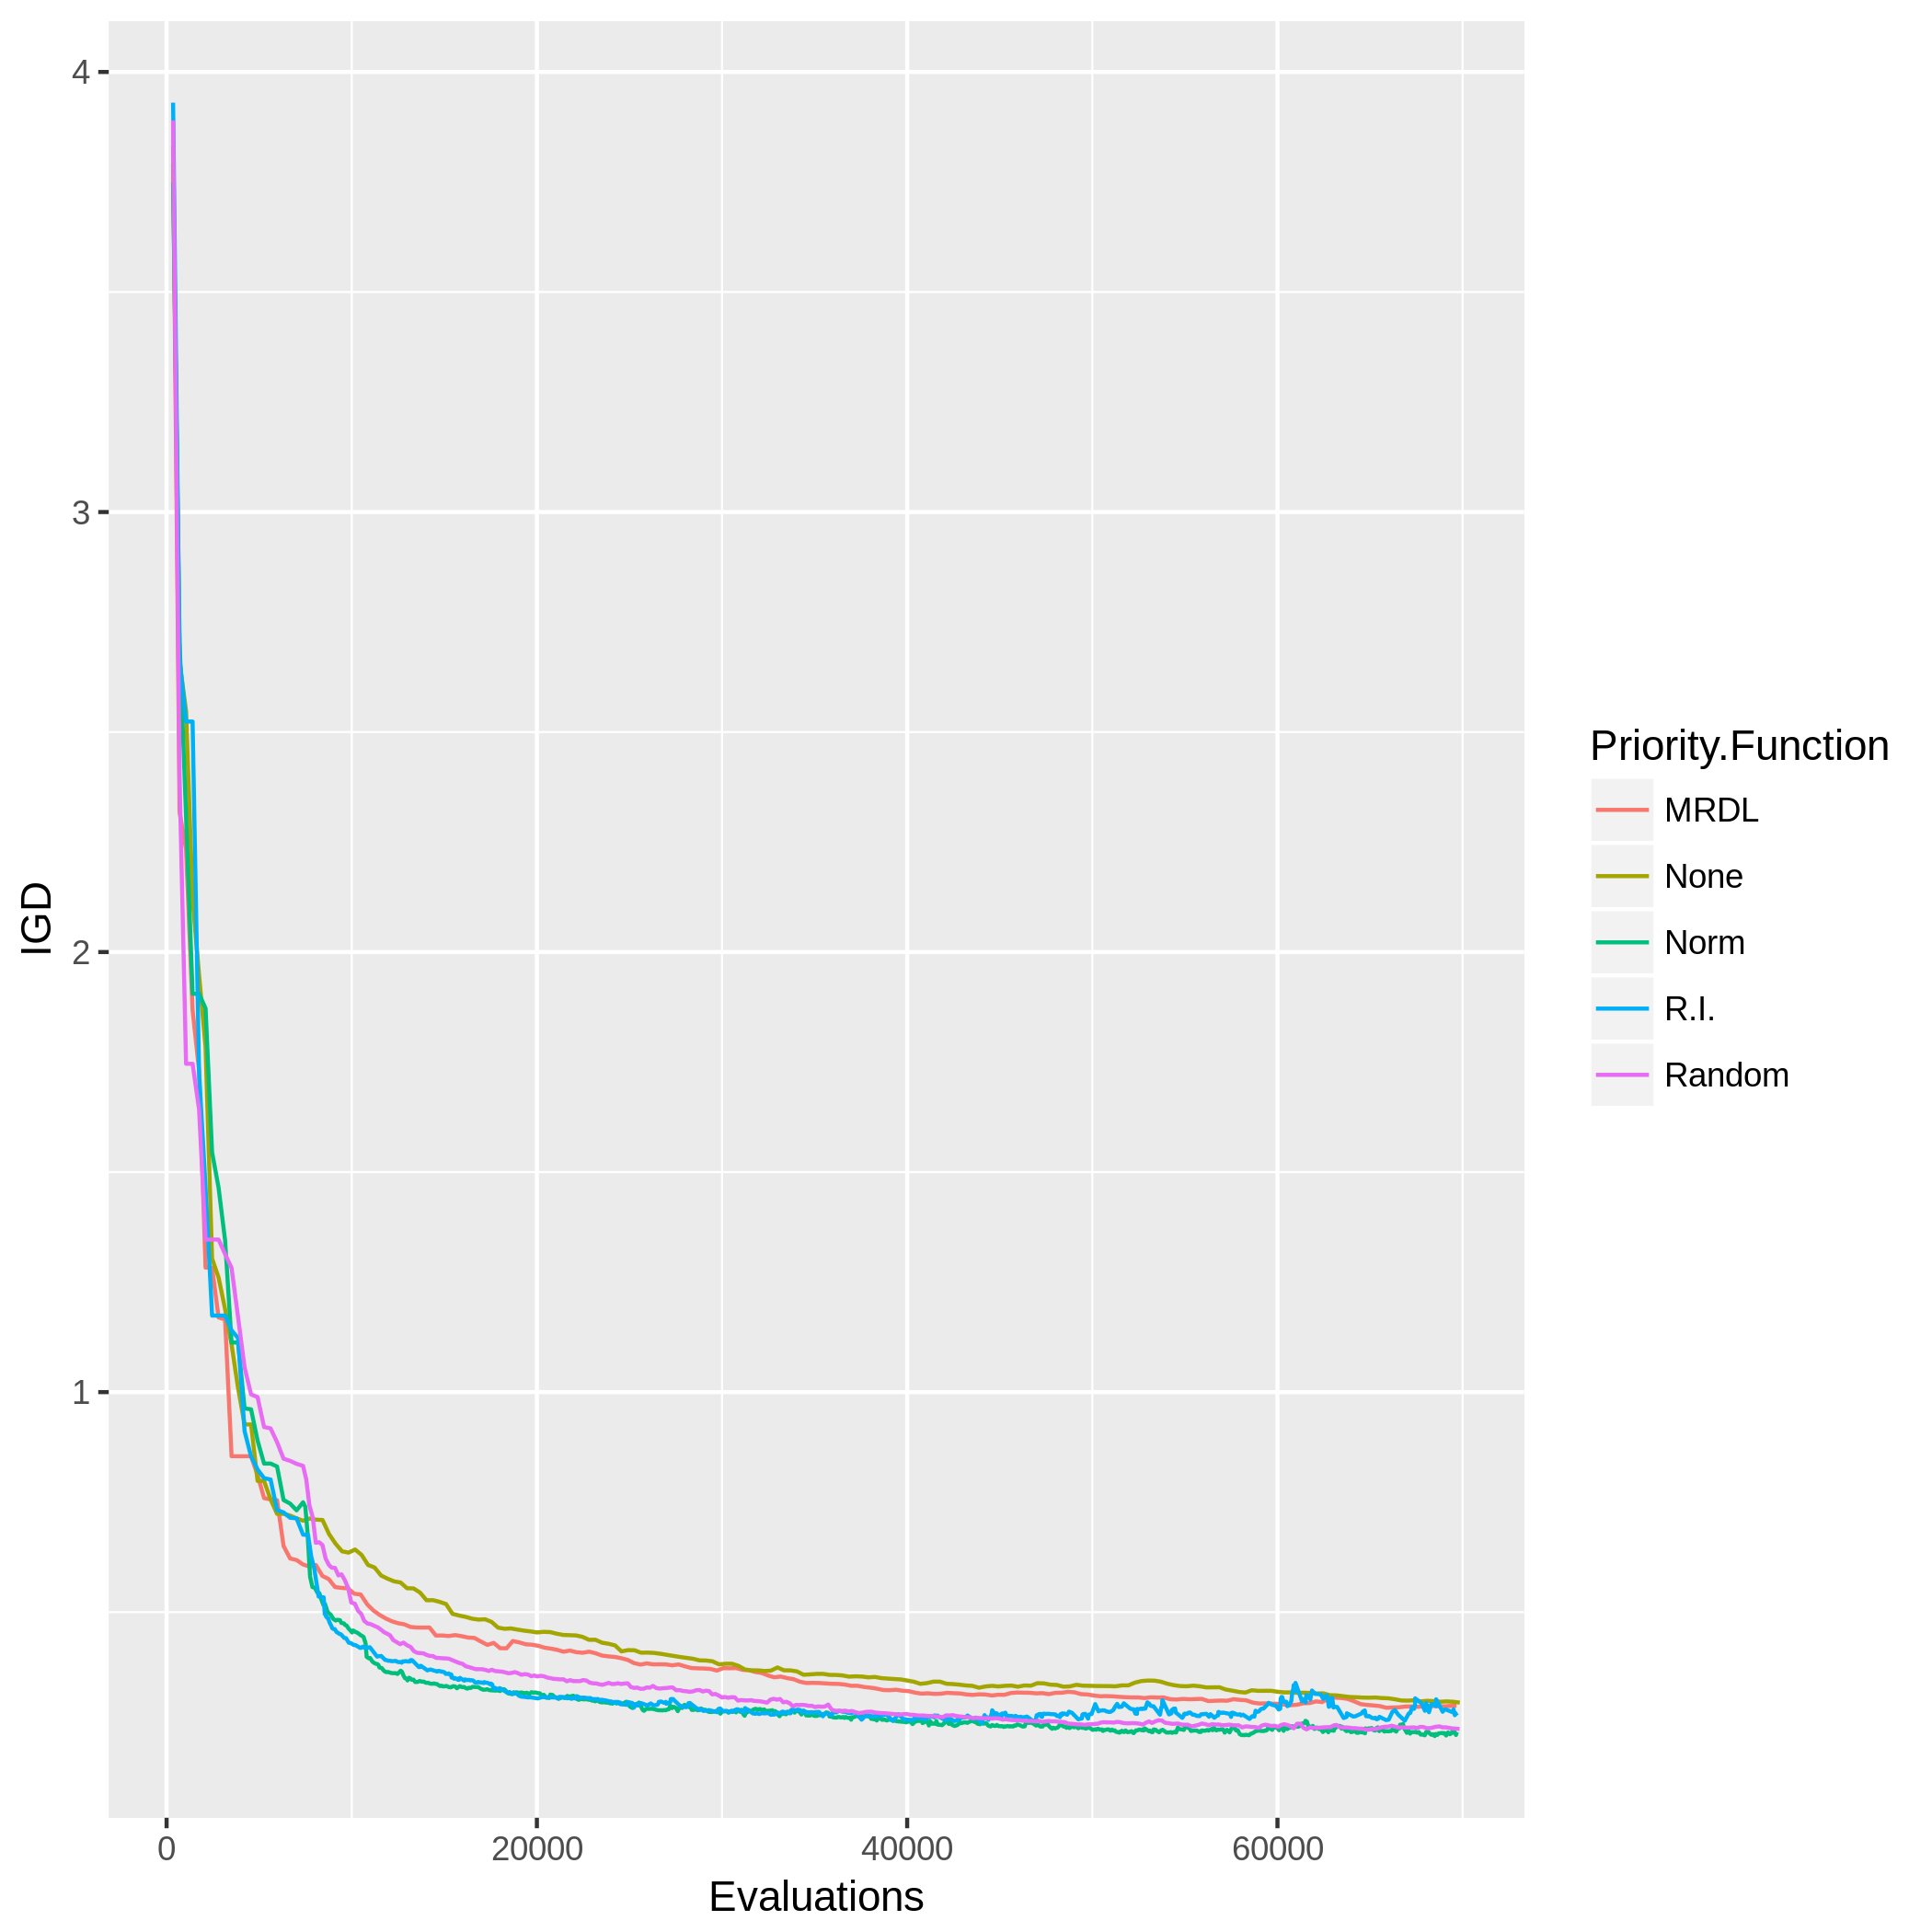
\includegraphics[width=1\textwidth, height=0.7\textwidth]{images/UF8igd_all}
			\caption{Evolution of the IGD on the UF8}
		\end{subfigure}
		\caption{SBX crossover - ($\lambda, \lambda$) scheme.}
			\label{evolution_igd}
	\end{figure*}


\begin{figure*}[!t]
	
	%	\Large{Average performance on different tournament size - Gallagher's Gaussian 21-hi Peaks Function}
	\begin{subfigure}[b]{0.33\textwidth}
		\centering
		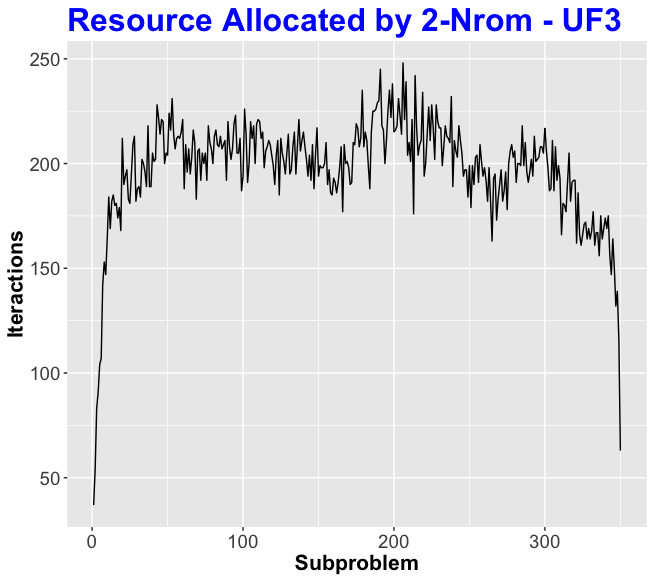
\includegraphics[width=1\textwidth, height=1\textwidth]{images/Ra-norm-uf3}
		\caption{RA}
	\end{subfigure}
	\begin{subfigure}[b]{0.33\textwidth}
		\centering
		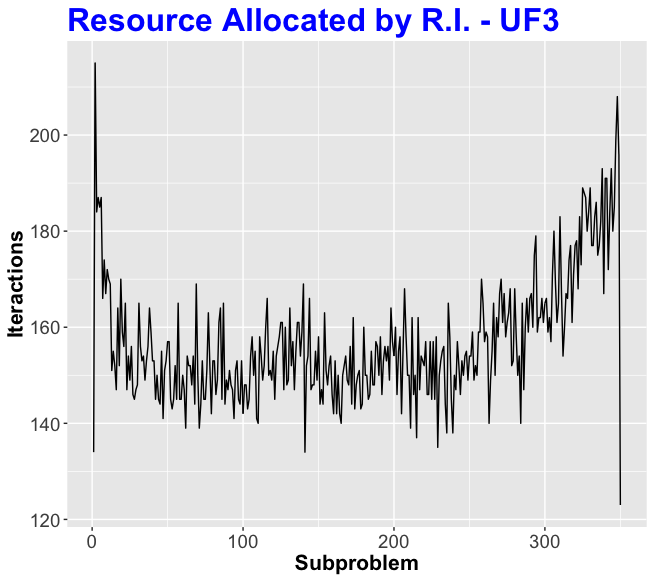
\includegraphics[width=1\textwidth, height=1\textwidth]{images/Ra-gra-uf3}
		\caption{RA}
	\end{subfigure}
	%	\begin{subfigure}[b]{0.33\textwidth}
	%		\centering
	%		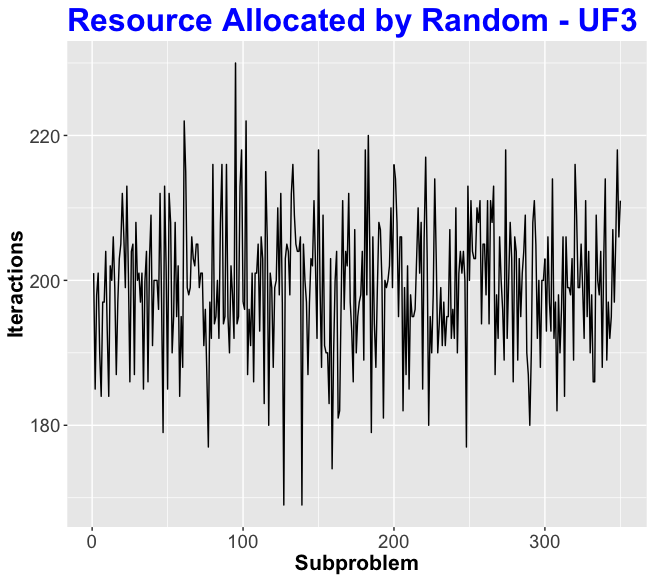
\includegraphics[width=1\textwidth, height=1\textwidth]{images/Ra-random-uf3}
	%		\caption{RA}
	%	\end{subfigure}
	\begin{subfigure}[b]{0.33\textwidth}
		\centering
		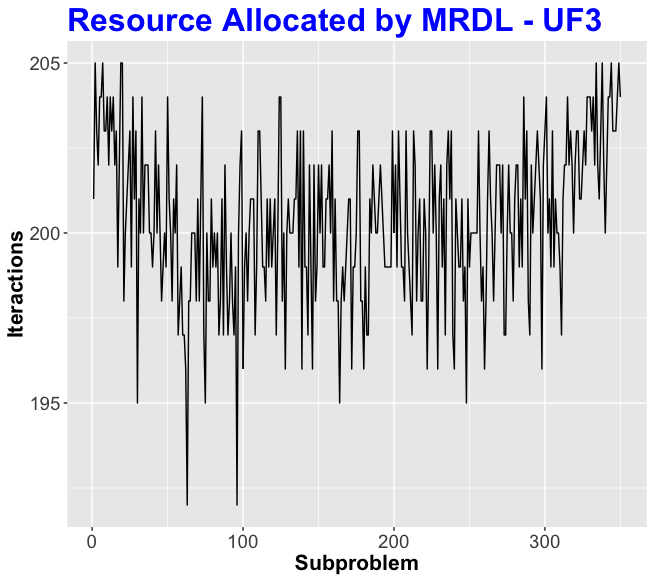
\includegraphics[width=1\textwidth, height=1\textwidth]{images/Ra-mrdl-uf3}
		\caption{RA}
	\end{subfigure}
	\caption{SBX crossover - ($\lambda, \lambda$) scheme.}
	\label{RAs - UF3}
	
\end{figure*}


\begin{figure*}[!t]
	
	%	\Large{Average performance on different tournament size - Gallagher's Gaussian 21-hi Peaks Function}
	\begin{subfigure}[b]{0.33\textwidth}
		\centering
		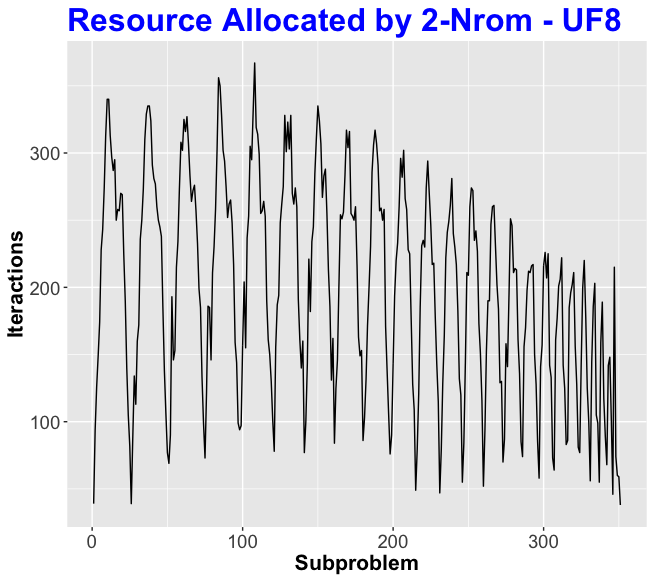
\includegraphics[width=1\textwidth, height=1\textwidth]{images/Ra-norm-uf8}
		\caption{RA}
	\end{subfigure}
	\begin{subfigure}[b]{0.33\textwidth}
		\centering
		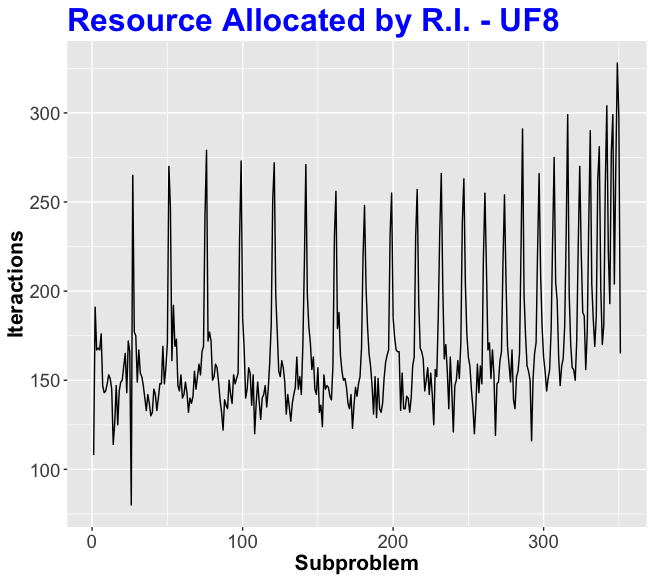
\includegraphics[width=1\textwidth, height=1\textwidth]{images/Ra-gra-uf8}
		\caption{RA}
	\end{subfigure}
	%	\begin{subfigure}[b]{0.33\textwidth}
	%		\centering
	%		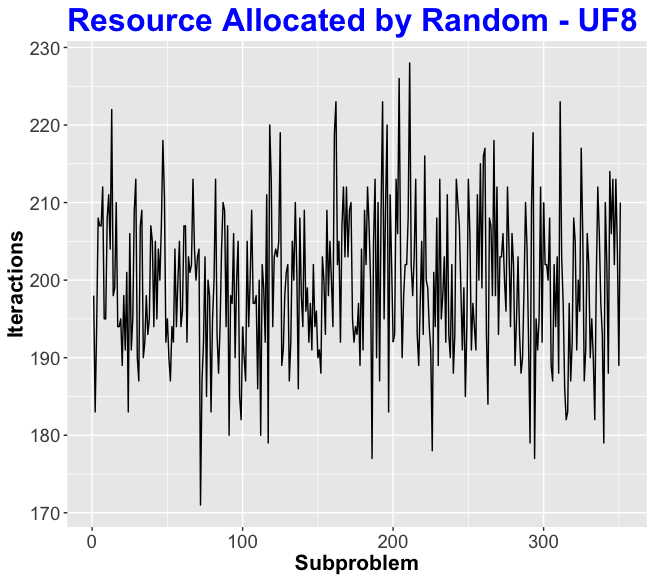
\includegraphics[width=1\textwidth, height=1\textwidth]{images/Ra-random-uf8}
	%		\caption{RA}
	%	\end{subfigure}
	\begin{subfigure}[b]{0.33\textwidth}
		\centering
		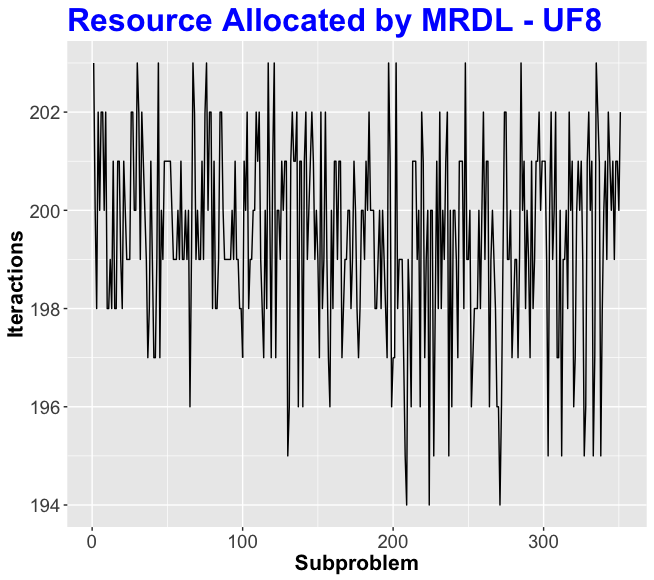
\includegraphics[width=1\textwidth, height=1\textwidth]{images/Ra-mrdl-uf8}
		\caption{RA}
	\end{subfigure}
	\caption{SBX crossover - ($\lambda, \lambda$) scheme.}
	\label{RAs - UF8}
	
\end{figure*}

\begin{table*}[!t]
	\begin{tabular}{llllll}
		\cline{6-6}
		\hline
		\rowcolor[gray]{.7} \multicolumn{1}{|l|}{PF:}         & \multicolumn{1}{l|}{None} & \multicolumn{1}{l|}{MRDL} & \multicolumn{1}{l|}{Norm} & \multicolumn{1}{l|}{R.I.} & \multicolumn{1}{l|}{Random} \\ \hline \hline
		\multicolumn{1}{|l|}{Lunar}           & \multicolumn{1}{l}{0.74 (0.10)} & \multicolumn{1}{l}{0.87 (0.11)} & \multicolumn{1}{l}{\textbf{0.93} (0.10)$*$} & 0.76 (0.08)             &\multicolumn{1}{l|} {0.76 (0.08)} \\ \hline \hline
		\rowcolor[gray]{.95} \multicolumn{1}{|l|}{UF1}              & \multicolumn{1}{l}{0.86 (0.02)} & \multicolumn{1}{l}{0.86 (0.01)} & \multicolumn{1}{l}{0.83 (0.02)} & \textbf{0.88 (0.01)$*$}             &\multicolumn{1}{l|} {\textbf{0.88 (0.01)$*$}} \\ \hline \hline
		\multicolumn{1}{|l|}{UF2}              & \multicolumn{1}{l}{0.75 (0.01)} & \multicolumn{1}{l}{0.75 (0.01)} & \multicolumn{1}{l}{ 0.76 (0.01)$*$} & \textbf{0.77 (0.08)$*$}             &\multicolumn{1}{l|} {\textbf{0.77 (0.01)$*$}} \\ \hline \hline
		\rowcolor[gray]{.95}\multicolumn{1}{|l|}{UF3}              & \multicolumn{1}{l}{0.84 (0.04)} & \multicolumn{1}{l}{0.86 (0.04)} & \multicolumn{1}{l}{ \textbf{0.94 (0.02)}$*$} & 0.92 (0.03)$*$             &\multicolumn{1}{l|}  {0.91 (0.04)$*$} \\ \hline \hline
		\multicolumn{1}{|l|}{UF4}              & \multicolumn{1}{l}{0.36 (0.01)} & \multicolumn{1}{l}{\textbf{0.37 (0.01)}} & \multicolumn{1}{l}{ \textbf{0.37 (0.01)}$*$} & \textbf{0.37 (0.01)$*$}             &\multicolumn{1}{l|} {\textbf{0.37 (0.01)$*$}} \\ \hline \hline
		\rowcolor[gray]{.95}\multicolumn{1}{|l|}{UF5}              & \multicolumn{1}{l}{0.63 (0.02)} & \multicolumn{1}{l}{0.66 (0.02)$*$} & \multicolumn{1}{l}{ 0.75 (0.03)$*$} & \textbf{0.81 (0.01)$*$}             &\multicolumn{1}{l|} {\textbf{0.81 (0.02)$*$}} \\ \hline \hline
		\multicolumn{1}{|l|}{UF6}              & \multicolumn{1}{l}{0.66 (0.02)} & \multicolumn{1}{l}{0.66 (0.01)} & \multicolumn{1}{l}{ 0.66 (0.02)} & \textbf{0.69 (0.01)$*$}             &\multicolumn{1}{l|} {\textbf{0.69 (0.01)$*$}} \\ \hline \hline
		\rowcolor[gray]{.95}\multicolumn{1}{|l|}{UF7}              & \multicolumn{1}{l}{0.80 (0.01)} & \multicolumn{1}{l}{0.80 (0.01)} & \multicolumn{1}{l}{ 0.82 (0.01)$*$} & \textbf{0.84 (0.01)$*$}             &\multicolumn{1}{l|} {0.83 (0.01)$*$} \\ \hline \hline
		\multicolumn{1}{|l|}{UF8}              & \multicolumn{1}{l}{0.89 (0.01)} & \multicolumn{1}{l}{0.90 (0.01)$*$} & \multicolumn{1}{l}{ 0.91 (0.01)$*$} & \textbf{0.92 (0.01)$*$}             &\multicolumn{1}{l|} {\textbf{0.92 (0.01)$*$}} \\ \hline \hline
		\rowcolor[gray]{.95}\multicolumn{1}{|l|}{UF9}              & \multicolumn{1}{l}{0.93 (0.01)} & \multicolumn{1}{l}{0.93 (0.01)} & \multicolumn{1}{l}{ \textbf{0.94 (0.01)$*$}} & 0.93 (0.01)             &\multicolumn{1}{l|} {\textbf{0.94 (0.01)$*$}} \\ \hline \hline
		\multicolumn{1}{|l|}{UF10}              & \multicolumn{1}{l}{079 (0.02)} & \multicolumn{1}{l}{0.78 (0.02)} & \multicolumn{1}{l}{ 0.83 (0.03)$*$} & \textbf{0.86 (0.03)$*$}             &\multicolumn{1}{l|} {0.84 (0.02)$*$} \\ \hline
	\end{tabular}
	\caption{HV Results - Lunar problem: The best algorithm is the one that uses Norm. It is the only one that is stats different from None, although by median all priority functions are better. Highlighted are the best values found.Star $*$ means stat diff from MOEA/D-DE without priority function. SD Values smaller than 0.01 were truncated to that\\ for UF the results are}
	\label{table_hv}
\end{table*}

\begin{table*}[!t]
	\begin{tabular}{llllll}
		\cline{6-6}
		\hline
		\rowcolor[gray]{.7} \multicolumn{1}{|l|}{PF:}         & \multicolumn{1}{l|}{None} & \multicolumn{1}{l|}{MRDL} & \multicolumn{1}{l|}{Norm} & \multicolumn{1}{l|}{R.I.} & \multicolumn{1}{l|}{Random} \\ \hline \hline
		\multicolumn{1}{|l|}{UF1}              & \multicolumn{1}{l}{0.14 (0.01)} & \multicolumn{1}{l}{0.13 (0.01)} & \multicolumn{1}{l}{0.10 (0.02)$*$} & \textbf{0.09 (0.01)$*$}             & \multicolumn{1}{l|} {\textbf{0.09 (0.01)$*$}} \\ \hline \hline
		\rowcolor[gray]{.95}\multicolumn{1}{|l|}{UF2}              & \multicolumn{1}{l}{0.08 (0.01)} & \multicolumn{1}{l}{0.08 (0.01)} & \multicolumn{1}{l}{ \textbf{0.06 (0.01)$*$}} & \textbf{0.06 (0.01)$*$}             & \multicolumn{1}{l|} {\textbf{0.06 (0.01)$*$}} \\ \hline \hline
		\multicolumn{1}{|l|}{UF3}              & \multicolumn{1}{l}{0.26 (0.01} & \multicolumn{1}{l}{0.26 (0.01)} & \multicolumn{1}{l}{ \textbf{0.17 (0.02)}$*$} & 0.18 (0.03)$*$             &  \multicolumn{1}{l|} {0.21 (0.03)$*$} \\ \hline \hline
		\rowcolor[gray]{.95}\multicolumn{1}{|l|}{UF4}              & \multicolumn{1}{l}{0.10 (0.01)} & \multicolumn{1}{l}{ 0.10 (0.01)} & \multicolumn{1}{l}{ \textbf{0.09 (0.01)}$*$} & \textbf{0.09 (0.01)$*$}             & \multicolumn{1}{l|} {\textbf{0.09 (0.01)$*$}} \\ \hline \hline
		\multicolumn{1}{|l|}{UF5}              & \multicolumn{1}{l}{1.75 (0.08)} & \multicolumn{1}{l}{1.65 (0.09)$*$} & \multicolumn{1}{l}{ \textbf{0.97 (0.06)$*$}} & 1.05 (0.06)$*$            & \multicolumn{1}{l|} {1.08(0.07)$*$} \\ \hline \hline
		\rowcolor[gray]{.95}\multicolumn{1}{|l|}{UF6}              & \multicolumn{1}{l}{0.12 (0.03)} & \multicolumn{1}{l}{0.12 (0.02)} & \multicolumn{1}{l}{ 0.10 (0.07)$*$} & \textbf{0.08 (0.01)$*$}            & \multicolumn{1}{l|} {\textbf{0.08 (0.02)$*$}} \\ \hline		 \hline
		\multicolumn{1}{|l|}{UF7}              & \multicolumn{1}{l}{0.12 (0.02)} & \multicolumn{1}{l}{0.13 (0.01)} & \multicolumn{1}{l}{ \textbf{0.06 (0.01)$*$}} & 0.07 (0.01)$*$             & \multicolumn{1}{l|} {0.07 (0.01)$*$} \\ \hline \hline
		\rowcolor[gray]{.95}\multicolumn{1}{|l|}{UF8}              & \multicolumn{1}{l}{0.29 (0.01)} & \multicolumn{1}{l}{0.28 (0.01)$*$} & \multicolumn{1}{l}{ \textbf{0.23 (0.01)$*$}} & 0.26 (0.02)$*$             & \multicolumn{1}{l|} {\textbf{0.23 (0.01)$*$}} \\ \hline \hline
		\multicolumn{1}{|l|}{UF9}              & \multicolumn{1}{l}{0.45 (0.01)} & \multicolumn{1}{l}{0.44 (0.01)$*$} & \multicolumn{1}{l}{ \textbf{0.39 (0.02)$*$}} & 0.42 (0.02)$*$             & \multicolumn{1}{l|} {0.40 (0.02)$*$} \\ \hline \hline
		\rowcolor[gray]{.95}\multicolumn{1}{|l|}{UF10}              & \multicolumn{1}{l}{3.69(0.20)} & \multicolumn{1}{l}{3.46 (0.0.23)$*$} & \multicolumn{1}{l}{ 2.38 (0.24)$*$} & \textbf{2.36 (0.27)$*$}             & \multicolumn{1}{l|} {2.64 (0.25)$*$} \\ \hline 
	\end{tabular}
	\caption{Highlighted are the best values found.Star $*$ means stat diff from MOEA/D-DE without priority function. SD Values smaller than 0.01 were truncated to that\\ for UF the results are}
	\label{table_igd}
\end{table*}

It is in our understand that using priority functions in both real-world and artificial benchmarks improve the results of MOEA/D-DE. For all group of functions the performance of MOEA/D-DE, in terms of HV or IGD median values, was always suppressed by at least one variation using priority functions. 

\subsection{UF benchmark functions}

Figure~\ref{HVS} (b) and (c) show box-plot that exemplify the results found in the UF benchmark functions in terms of the HV values while Figure~\ref{IGDS} (a) and (b) does the same but in terms of the IGD values. In it we can see that MRDL as a priority function is slightly better than MOEA/D-DE in terms of median and standard deviation.  With R.I., 2-Norm and Random performing the best.

Turning to the results of the Tables~\ref{table_hv} and ~\ref{table_igd}, we discuss the results of every priority function. The 2-norm as priority function lead to several good results in median of the HV values while had very good results in the median of the IGD values. We highlight in the UF-5 function, being clearly better than the others. The relative improvement function was first introduced in the context of the unconstrained MOEA competition in the CEC 2009~\cite{zhang2009performance}, being the winner of that competition~\cite{zhang2008multiobjective}. This competition introduced the UF benchmark functions, so it came to us with no surprising the good results from the relative improvement priority function. In terms of HV values, in all but in the UF-3 and UF-9 benchmark function it had the best result, being significantly different from the MOEA/D-DE in every single case. The results of the relative improvement in terms of median values of the IGD values was not as remarkable, but they are still very good. For our great surprise the Random priority function performed quiet well (and better than the MRDL). 

 Figures~\ref{evolution_hv} (b) and (c) and~\ref{evolution_igd} (a) and (b) show how the values of the HV and IGD evolve over the iteractions of the algorithms. For the UF-3 function the results caught our attention. First, it seems that more evaluations are need to a convergence of the values. Second, for the HV values the priority functions relative improvement and 2-norm made a "jump" over 30000 and 60000 evaluations, improving fast the HV metric values. Also at the end fo the evaluations, there is a strange regressive peak of the HV and IGD values of the 2-Norm. That said, in most cases the values of HV and IGD converged by the end of the number evaluations (70000).

\subsection{DTLZ benchmark functions}



\subsection{Lunar Landing Problem}


Figure~\ref{HVS} (a) show box-plot the results found in the Lunar Landing benchmark problem in terms of the HV values. Both priority functions related to diversity, MRDL and 2-norm, improved a lot the performance of the MOEA/D-DE. On the other hand, the relative improvement lead to a diminish of the standard deviation, with just a slight improvement on the performance.  Figure~\ref{evolution_hv} (a) show how the values of the HV evolve over the iteractions of the algorithms. All of the variants had converged around 20000 evaluations, with the exception of the MRDL (it converged with 40000). All used around half or less of the total number evaluations (70000) to converge.

Changing to the results of the Table~\ref{table_hv}, we discuss the results of medians and standard deviation the priority functions.  We highlight the outstanding result of 2-norm since it was clearly better than the other priority function results in terms of median of HV values as it is statistically different from MOEA/D-DE, yet its standard deviation was very high. The results of MRDL were not as good as the previous one, however, it is still had impressive median HV values results, but without statistically significant difference from MOEA/D-DE. The relative improvement improved the results of MOEA/D-DE but not as much as in the case of the UF benchmark functions, where it had frequently the best results. Here, on the other hand, the main improvement was in terms of diminishing the standard deviation. The random priority function performed poorly. More results can be found at the supplementary materials.

\subsection{Resource Allocation}

